% ============================================================================
% FLAIME --- DOE Genesis Mission Phase I Proposal Template
% DE-FOA-0003612: The Genesis Mission: Transforming Science and Energy with AI
% Topic 3, Focus Area B: AI-Enabled Materials Discovery and Engineering
%                         (AMMTO)
% ============================================================================
%
% STRUCTURE (per FOA Section IV.C):
%   Field 7: Project Summary / Abstract (1 page, via Grants.gov)
%   Field 8: Single PDF containing:
%     - DOE Title Page (does NOT count against 5-page limit)
%     - Project Narrative (5 pages maximum)
%     - Appendix 1: Bibliography & References Cited
%     - Appendix 2: Facilities & Other Resources (0.5 page max)
%     - Appendix 3: Equipment (0.5 page max)
%     - Appendix 4: DMSP (NOT required at submission; required at award)
%     - Appendix 5: Synergistic Activities (optional, 1 page per person)
%     - Appendix 6: Transparency of Foreign Connections
%     - Appendix 7: Other Attachments (Letters of Commitment, etc.)
%   Senior/Key Person Profile (Expanded) form:
%     - Biographical Sketches (SciENcv)
%     - Current and Pending Support (SciENcv)
%   SF-424 R&R Budget form + Budget Justification
%
% TOGGLE TODO NOTES:
%   With instructions visible:   \usepackage{todonotes}
%   Clean output (no notes):     \usepackage[disable]{todonotes}
% ============================================================================

\documentclass[11pt,letterpaper]{article}

% --- Page geometry (FOA: 1-inch margins, letter paper) ---
\usepackage[margin=1in]{geometry}

% --- Fonts and encoding ---
\usepackage[T1]{fontenc}
\usepackage[utf8]{inputenc}
\usepackage{mathptmx}          % Times Roman (DOE-preferred serif font, >= 11pt)

% --- Math and symbols ---
\usepackage{amsmath,amssymb}
\usepackage{textcomp}          % For \textdegree and other symbols
\usepackage{siunitx}           % For \num{} number formatting

% --- Graphics and figures ---
\usepackage{graphicx}
\graphicspath{{figures/}{figures/equipment/}}
\usepackage[table]{xcolor}
\usepackage{float}             % For [H] placement
\usepackage{wrapfig}           % For inline equipment images

% --- Tables ---
\usepackage{booktabs}
\usepackage{tabularx}

% (lipsum package removed — no longer needed)

% --- Lists ---
\usepackage{enumitem}
\setlist{nosep,leftmargin=*}

% --- Bibliography (natbib must load before hyperref) ---
\usepackage[numbers,sort&compress]{natbib}

% --- References and links ---
\usepackage[
  colorlinks=true,
  linkcolor=blue!70!black,
  citecolor=blue!70!black,
  urlcolor=blue!70!black
]{hyperref}

% --- Headers and footers ---
\usepackage{fancyhdr}
\pagestyle{fancy}
\fancyhf{}
\renewcommand{\headrulewidth}{0.4pt}
\lhead{\small FLAIME --- DE-FOA-0003612 --- Topic~3-B}
\rhead{\small Phase~I}
\cfoot{\thepage}

% --- Section formatting ---
\usepackage{titlesec}
\titleformat{\section}{\normalfont\large\bfseries}{\thesection.}{0.5em}{}
\titleformat{\subsection}{\normalfont\normalsize\bfseries}{\thesubsection.}{0.5em}{}
\titlespacing*{\section}{0pt}{1.2ex plus 0.4ex minus 0.2ex}{0.8ex plus 0.2ex}
\titlespacing*{\subsection}{0pt}{0.8ex plus 0.3ex minus 0.1ex}{0.5ex plus 0.1ex}

% --- Paragraph spacing (tight for 5-page limit) ---
\setlength{\parindent}{0pt}
\setlength{\parskip}{4pt plus 1pt minus 1pt}

% --- Caption formatting ---
\usepackage[font=small,labelfont=bf]{caption}

% --- Build mode toggles ---
% Three build targets from a single source file:
%   make draft     -> annotated PDF (watermark + todonotes + all sections)
%   make clean-pdf -> clean PDF (no watermark, no notes, all sections)
%   make final     -> submission-ready Field 8 PDF (removes abstract, biosketch, budget)
%
% Override at build time via \def:
%   \cleanbuild   -> disables draft watermark and todonotes
%   \submissionbuild -> also excludes non-Field-8 sections (abstract, biosketches, budget)
\newif\ifdraft
\newif\ifsubmission
\ifdefined\submissionbuild
  \draftfalse
  \submissiontrue
\else\ifdefined\cleanbuild
  \draftfalse
  \submissionfalse
\else
  \drafttrue
  \submissionfalse
\fi\fi

\ifdraft
  \usepackage{draftwatermark}
  \SetWatermarkText{DRAFT}
  \SetWatermarkScale{4}
  \SetWatermarkColor[gray]{0.92}
\fi

% =========================================================================
% TODO NOTES --- controlled by \ifdraft toggle above
% =========================================================================
\ifdraft
  \usepackage{todonotes}
\else
  \usepackage[disable]{todonotes}
\fi

% Custom note styles for different instruction types:
%   \instruct{...}  --- Writing instructions (orange, inline)
%   \guidance{...}  --- Strategic/framing guidance (blue, inline)
%   \required{...}  --- FOA-required content flag (red, inline)
%   \note{...}      --- General authoring notes (green, inline)
\newcommand{\instruct}[1]{\todo[inline,color=orange!30]{#1}}
\newcommand{\guidance}[1]{\todo[inline,color=blue!20]{#1}}
\newcommand{\required}[1]{\todo[inline,color=red!25,bordercolor=red!60]{%
  \textbf{REQUIRED:} #1}}
\newcommand{\note}[1]{\todo[inline,color=green!20]{#1}}

% --- Other custom commands ---
\newcommand{\flaime}{\textsc{Flaime}}
\newcommand{\bofn}{\textsc{Bofn}}
\newcommand{\projecttitle}{\flaime{} (Fast Learning AI for Mineral
Efficiency): Autonomous Discovery and Qualification of
Critical-Mineral-Lean Alloys for Clean Energy}
\newcommand{\pagebudget}[1]{\ifdraft\hfill\textcolor{blue!60!black}{\footnotesize%
  \textsf{[\,$\sim$#1\,page\ifx#11\else s\fi]}}\fi}

% --- Element palette and sub-system parameters (single source of truth) ---
% The palette lists non-Al alloying additions; Al is always the base element.
% k = number of alloying elements chosen; k=2 → ternary (Al + 2), k=3 → quaternary, etc.
\usepackage{etoolbox}  % for \docsvlist / \appto auto-derivation
% ── Element Palette (single source of truth) ──────────────────────────
% EDIT ONLY the three lines marked ★; everything else auto-derives at compile time.
%
% After editing \elementpalette, \kmin, or \kmax, recompute \subsystemcount:
%   python3 -c "
%   from math import comb
%   elems = 'Mn,Cr,Zr,Mg,Si,Cu,Ti,Fe,Ni,Ce,Sc,Li,Er,Zn,Sn'.split(',')
%   n = len(elems); kmin = 2; kmax = 8
%   total = sum(comb(n,k) for k in range(kmin, kmax+1))
%   print(f'elementcount={n}, subsystems={total}')
%   "
%   Current output: elementcount=15, subsystems=22803
%
\newcommand{\elementpalette}{Mn,Cr,Zr,Mg,Si,Cu,Ti,Fe,Ni,Ce,Sc,Li,Er,Zn,Sn} % ★ canonical comma-list
\newcommand{\kmin}{2}                    % ★ minimum additions per sub-system (k=2 → ternary)
\newcommand{\kmax}{8}                    % ★ maximum additions per sub-system (k=8 → 9-component)
%
% --- Auto-derived: element count (compile-time) ---
\newcounter{elemctr}
\setcounter{elemctr}{0}
\renewcommand*{\do}[1]{\stepcounter{elemctr}}
\expandafter\docsvlist\expandafter{\elementpalette}
\newcommand{\elementcount}{\theelemctr}  % auto-counted: currently 15
%
% --- Auto-derived: "Mn, Cr, Zr, ..." human-readable list (compile-time) ---
\def\elementlist{}
\newif\iffirstlistelem\firstlistelemtrue
\renewcommand*{\do}[1]{%
  \iffirstlistelem\firstlistelemfalse\appto\elementlist{#1}%
  \else\appto\elementlist{, #1}\fi}
\expandafter\docsvlist\expandafter{\elementpalette}
%
% --- Auto-derived: "Mn,\,Cr,\,Zr,\,..." LaTeX thin-space list (compile-time) ---
\def\elementlisttex{}
\firstlistelemtrue
\renewcommand*{\do}[1]{%
  \iffirstlistelem\firstlistelemfalse\appto\elementlisttex{#1}%
  \else\appto\elementlisttex{,\,#1}\fi}
\expandafter\docsvlist\expandafter{\elementpalette}
%
% --- Sub-system count (recompute with script above when palette changes) ---
\newcommand{\subsystemcount}{22\,803}    % = sum C(\elementcount,k) for k=\kmin..\kmax
\newcommand{\subsystemcountraw}{22803}   % raw integer

% ============================================================================
\begin{document}

% ============================================================================
%  PART 0: PROJECT SUMMARY / ABSTRACT  (Field 7, Grants.gov, 1 page max)
% ============================================================================
\ifsubmission\else  % Abstract is Field 7 (Grants.gov) --- exclude from Field 8 PDF
%
% NOTE: The abstract is submitted via Field 7 on the SF-424 R&R Other
% Project Information form in Grants.gov --- NOT inside the Project
% Narrative PDF.  It is reproduced here for drafting convenience only.
% Delete this section before assembling the final Field 8 PDF.
%
% ============================================================================
\section*{Project Summary / Abstract}
\label{sec:abstract}
\thispagestyle{empty}

\required{FOA \S IV.C, Field 7: The abstract is entered via Grants.gov
(Field 7 on the R\&R Other Project Information form), NOT in the Project
Narrative PDF.  This page is for drafting only --- remove before final
assembly of the Field 8 file.}

\guidance{The abstract must include: (1)~project title, PI name and
affiliation, co-investigators and affiliations (these do not count against
the 1-page limit); (2)~a statement of the project's vision for the
science and applied energy initiatives; (3)~a description of how and why
AI will enhance the workflows.  Must fit on 1 page excluding the
investigator list (11pt, 1-in margins).  ``Suitable for distribution to
the public.'' Write this section LAST but polish heavily.}

\textbf{Project Title:} \projecttitle{}

\textbf{PI:} Sterling G.\ Baird, Ph.D., Brigham Young University

\textbf{Application Stage:} Phase I

\textbf{Senior/Key Personnel and Partner Organizations:}
Valimet Inc.\ (funded): Valimet's CTO, Valimet's technical manager---gas atomization;
AMAZEMET (funded): Amazemet's CEO, Amazemet's application engineer---ultrasonic atomization;
Thermo-Calc AB (funded): a Thermo-Calc specialist, Thermo-Calc's account manager---CALPHAD databases

\bigskip

The United States imports 100\% of its manganese, 100\% of its zirconium
mineral concentrates, and 74\% of its chromium~(USGS, 2024)---elements
central to high-performance aluminum alloys for advanced manufacturing. A single supply disruption could idle domestic
additive-manufacturing production dependent on these materials. FLAIME (Fast
Learning AI for Mineral Efficiency) addresses this vulnerability with an
AI-autonomous closed-loop platform that discovers and qualifies aluminum alloys
meeting structural performance targets while minimizing critical mineral
content, directly supporting DOE Critical Materials Strategy Pillars~2
(Develop Alternatives) and~3 (Materials and Manufacturing Efficiency).

FLAIME integrates Bayesian Optimization over Function Networks (BOFN) with
the partial Knowledge Gradient for Function Networks (pKGFN) acquisition
function to jointly optimize alloy composition, printability, and mechanical
properties across the full powder-to-part pipeline---from CALPHAD evaluation
through ultrasonic and gas atomization, laser powder bed fusion (LPBF),
and a staged minimum-viable-specimen (MVS) progression---single tracks,
density cubes ($\geq$99\% relative density gate), and ASTM~E8 sub-size
tensile bars. By modeling every manufacturing stage as a node in
a cost-aware function-network directed acyclic graph (DAG) with an embedded mineral-burden objective,
BOFN selects maximally informative experiments at each stage, reducing
powder-to-tensile cycle time by an estimated 10$\times$ versus conventional
sequential campaigns ($\geq$3$\times$ from AI-guided experiment
selection $\times$ ${\sim}$3$\times$ from closed-loop execution speedup)---software-orchestrated with human operators in Phase~I,
architected for direct robotic integration in Phase~II.  No existing
platform closes this complete composition-discovery and
manufacturing-qualification loop: the closest structural-alloy SDL
automates printing through testing but not the full
powder-to-property pipeline~(Conn et~al., 2025).

Phase~I explores \subsystemcount{} element combinations---$\sum_{k=2}^{8}\binom{\elementcount}{k}$
sub-systems spanning ternary (e.g., Al--Fe--Si) through 9-component alloys---drawn from a
\elementcount-element Al-alloy palette via an asynchronous, cost-aware multi-fidelity
framework (\texttt{pycalphad}, TC-Python/TCAl10, Thermo-Calc AM~Module)
that evaluates CALPHAD thermodynamics, Scheil solidification, and
printability in parallel at maximum high-performance computing (HPC) capacity,
then focuses experimental validation on the top 3--6 sub-systems---including
the Al--Mn--Cr--Zr and Al--Zr initial focus systems---characterizing 100--200 compositions
(up to 3~compositions/day M--F and 1 on Saturday, ${\leq}16$/week) through the full
powder-to-tensile pipeline with a discovery yield $\geq$3\% (at least 3--6 high-performing alloys). All
experimental data and BOFN models will be shared as a FAIR-compliant
digital thread via the Genesis Mission platform and open repositories
(Zenodo/Figshare with DOIs). The project enters Phase~I at
TRL~2 (concept formulated) and targets TRL~4 (closed-loop validated in
laboratory) at the conclusion of the 9-month, \$750K effort.

\newpage
\fi % end \ifsubmission\else (abstract)

% ============================================================================
%  PART 1: DOE TITLE PAGE  (does NOT count against 5-page limit)
% ============================================================================
\section*{DOE Title Page}
\label{sec:titlepage}
\thispagestyle{empty}

\required{FOA \S IV.C: ``The material listed here defines the required
content of a title page. Additional material is not allowed.''  Use the
Excel template from Grants.gov ``Related Documents'' tab for the budget
summary portion.}

\begin{center}
\textbf{Project Title:}\\
\projecttitle{}

\bigskip

\textbf{Lead Applicant/Institution:} Brigham Young University (BYU)\\
\textbf{Street Address:} 701 E University Parkway, 350 EB, Provo, UT 84602\\
\textbf{Postal Address:} Same as street address\\
\textbf{Lead PI:} Sterling G.\ Baird, Ph.D.\
  \textbar\ (801) 422-5344
  \textbar\ \href{mailto:sterling.baird@byu.edu}{sterling.baird@byu.edu}\\
\textbf{Administrative POC:} BYU research administration
\\
\textbf{RFA Number:} DE-FOA-0003612\\
\textbf{Challenge and Focus Area:}
  3-B Securing America's Critical Minerals Supply |
  AI-Enabled Materials Discovery and Engineering
\end{center}

\bigskip

\instruct{Fill in the Senior/Key Personnel table.  Must list ALL
partner institutions and their key personnel.}

\begin{table}[H]
\centering\small
\caption*{\textbf{Senior/Key Personnel}}
\begin{tabularx}{\textwidth}{lX}
\toprule
\textbf{Institution} & \textbf{Senior/Key Personnel} \\
\midrule
BYU (Lead) & S.\ G.\ Baird (PI); 2 MS students, 10 undergraduate researchers \\
Valimet (Funded Partner) & Valimet's CTO; Valimet's technical manager --- gas atomization \\
AMAZEMET (Funded Partner) & Amazemet's CEO; Amazemet's application engineer --- ultrasonic atomization \\
Thermo-Calc AB (Funded Partner) & a Thermo-Calc specialist; Thermo-Calc's account manager --- CALPHAD databases \\
\bottomrule
\end{tabularx}
\end{table}

\instruct{Fill in the budget summary table.  Use the Excel template from
Grants.gov ``Related Documents'' tab and attach to Field 12.  Include ALL
partner institutions whether or not they receive DOE funds.}

\begin{table}[H]
\centering\small
\caption*{\textbf{Summary Budget Information}}
\begin{tabularx}{\textwidth}{Xr}
\toprule
\textbf{Institution} & \textbf{Year 1 Budget (\$)} \\
\midrule
BYU (Lead) & 600,000 \\
Valimet (Funded Partner) & --- \\
AMAZEMET (Funded Partner) & --- \\
Thermo-Calc AB (Funded Partner) & --- \\
\midrule
\textbf{Total} & \textbf{750,000} \\
\bottomrule
\end{tabularx}
\end{table}

\newpage

% ============================================================================
%  PART 2: PROJECT NARRATIVE  (5 pages maximum --- FOA Section IV.C)
% ============================================================================
%
%  FOA-prescribed organization (strongly encouraged):
%    1. Background/Introduction          ~1   page
%    2. Project Objectives               ~0.5 page
%    3. Proposed Research and Methods     ~1.5 pages
%    4. Milestones in the Nine Months     ~1   page
%    5. Data Sources and Models           ~0.5 page
%    6. Decision Gate Metrics             ~0.5 page
%                                        ----------
%                               TOTAL:    5   pages
%
%  Figures, tables, charts, photos ALL count against the 5-page limit.
%  References, appendices, title page, and budget do NOT.
% ============================================================================

\setcounter{page}{1}  % Restart page counter for Project Narrative

\required{FOA \S IV.C: ``The Project Narrative must not exceed a page
limit of 5 pages of technical information, including charts, graphs,
maps, photographs, and other pictorial presentations.'' 11pt minimum,
1-in margins, letter paper.  Merit reviewers will ONLY consider the
first 5 pages.}

\required{FOA \S IV.C (p.71--72): ``Applicants must disclose the use
of any artificial intelligence tools in applications, unless the tools
were used solely for editing an original draft.''  Include a brief
disclosure statement, e.g., at the end of the narrative or in the
cover letter.}

\required{FOA \S IV.C (p.70): ``Do not include any websites (URLs)
that provide supplementary or additional information that constitutes
a part of the application.''  URLs to published papers or DOE pages
are fine; no external supplementary material.}

\required{FOA \S II.E (p.10): Phase I teams must include institutions
from at least 2 of the following 3 categories: (1) DOE/NNSA National
Laboratory or Scientific User Facility, (2) Industry, (3)
IHE/Non-profit/Other.  Verify team composition satisfies this requirement.}

\required{FOA \S IV.C (p.72): ``Each institution in a
multi-institutional team submitting collaborative applications must
submit an identical common narrative, including all appendices.''
Coordinate identical PDF assembly across all partners.}

\required{FOA \S IV.C (p.72): ``Biographical sketches and current and
pending support may no longer be provided as attachments to a Project
Narrative.'' These go on the Senior/Key Person Profile form ONLY.}

\guidance{REVIEW CRITERIA MAPPING (FOA \S VI.B, in descending
importance): (1)~Scientific/Technical Merit \& Impact $\to$ \S1
Background, \S6 Decision Gates; (2)~Technical Approach/Feasibility
$\to$ \S3 Methods, \S4 Milestones; (3)~Team/Resources/Management $\to$
\S3 (PI attribution), App.\ 2 Facilities; (4)~Commercialization
Potential $\to$ embed in \S6 and \S1; (5)~Budget/Cost-Effectiveness
$\to$ Budget Justification.  Allocate page space proportionally to
criterion weight.}

\guidance{FIGURE/TABLE STRATEGY: With 5 pages and all visuals counting
against the limit, budget up to 4 figures + 1 table ($\sim$1.6--2.0
pages).  Contingency if overflow: (A) drop Fig.~3 composite,
(B) merge Fig.~4 tensile into Fig.~2, (C) shrink Table~1 to 3 KPIs.
Text budget: $\sim$1,600 words.  Approximately 500 words/page at 11pt
Times.}

\guidance{GENESIS MISSION INTEGRATION (FOA p.13, p.70): Teams ``are
expected to take advantage of the [Genesis Mission] platform when
practical, including by hosting data, models, and other artifacts on
the platform'' and participate in coordination activities.  Reference
AmSC (American Science Cloud) and ModCon integration where applicable.
Applicants are encouraged to ``build upon general-purpose capabilities,
especially those produced by the Genesis Mission teams, building
domain-specific capabilities deployable in a plug-and-play fashion.''}

\guidance{WORD-COUNT BUDGET ($\sim$1{,}570 words body text + 4 figures + 1 table,
targeting $\sim$4.8 of 5 pages):
\S1~Background $\sim$300w, \S2~Objectives $\sim$250w,
\S3~Methods $\sim$400w, \S4~Milestones $\sim$200w + table,
\S5~Data $\sim$160w, \S6~Gates $\sim$180w, buffer $\sim$80w.
Track word count continuously --- the 5-page limit with figures counting
is the most common failure mode for Genesis Mission proposals.}

% --- 1. Background / Introduction (~1 page) --------------------------------
\section{Background and Introduction}\pagebudget{1}
\label{sec:background}

\guidance{FOA: ``Explain the importance and relevance of the proposed
work and clearly articulate which aspect of the chosen challenge will be
addressed and solved.  Set the proposed research in perspective to other
efforts in the field.  Highlight novel or unique aspects of the proposed
work.  Cite relevant literature.''  CRITICAL: Lead with the platform
need and AI advantage, not the alloy system.  Frame for Focus Area B
(AMMTO): autonomous discovery platforms, closed-loop AI, accelerated
qualification, reducing demand for critical minerals.}

\note{Buy America compliance statement below --- required within the
first 2 pages of the Project Narrative (FOA \S IV.C).}

\textbf{Overview.}
Manganese and zirconium are 100\% import-reliant and chromium 74\%
(USGS 2024~\cite{usgs_mcs_2024})---a single supply disruption could
idle U.S.\ AM production dependent on these
elements~\cite{bauer_2023_1998242}.  We propose \flaime{} (Fast Learning
AI for Mineral Efficiency), a Level~3 self-driving laboratory (SDL) in
the taxonomy of Tom et al.~\cite{tom_2024_acschemr}---a closed-loop,
AI-guided platform in which software selects experiments autonomously
while a small set of defined human handoffs execute physical
transfers---that will discover LPBF aluminum alloys meeting structural
performance targets while minimizing critical mineral content.  Related
efforts exist but none yet \emph{unify powder production, LPBF printing,
and tensile testing under a single AI decision loop with autonomous
sub-system selection}:
APEX envisions the automation of DED through mechanical characterization
(hardness measurements and compression testing) but has not been
publicly demonstrated in peer-reviewed work and reports sparse
implementation details~\cite{conn_2025_apex}; A-Lab targets oxides, not structural
metals~\cite{szymanski_2023_s4158602}; AMASE closes an
experiment--theory loop on thin-film phase maps, not bulk
parts~\cite{liang_2025_sciadvad}; DED-based active-learning
platforms discover bulk alloys at $>$100/week but use purchased
feedstocks without LPBF or tensile
qualification~\cite{nelaturu_2024_jmsea202}; BIRDSHOT demonstrates
closed-loop multi-objective BO with real mechanical testing but on a
pre-selected refractory system via arc
melting~\cite{paramore_2025_jactamat}; ICME-anchored closed-loop Al
alloy design for AM has been demonstrated but within expert-selected
systems~\cite{thapliyal_2020_jmtla201}; and recent BO-guided CALPHAD
work optimizes within a single expert-selected Al system using purely
computational objectives~\cite{glaser_2025_jmps106120}.  A recent
autonomy framework confirms that high software and hardware autonomy
have not yet been jointly achieved for structural
AM~\cite{tobias_2025_autonomy}.  By closing this \emph{decision} loop
via a complete powder-to-print-to-test pipeline---unifying
computational evaluation, powder atomization, laser powder bed fusion
(LPBF), and mechanical testing---\flaime{} targets a measurable
AI acceleration factor of $\geq$3$\times$ over conventional alloy
development for the decision-making portion (informed-prior Bayesian
optimization with cross-fidelity transfer; consistent with
${>}$3--5$\times$ speedups reported for closed-loop materials campaigns,
e.g.~\cite{liu_2024_llambo,paramore_2025_jactamat}), compounding with
closed-loop execution speedup from hardware and software automation of
the powder-to-print-to-test pipeline (automated AutoTrickler powder
dosing, scripted atomizer recipes, LPBF build-file generation, and
orchestrated transfer between build, prep, and test stations) for an
estimated ${\sim}$10$\times$ total reduction in discovery
time~\cite{tom_2024_acschemr}.%
\footnote{Buy America compliance statement (FOA \S IV.D.3, Build America,
Buy America Act certification): retained here pending PI confirmation
that it is required for Phase~I applications of this FOA; strike if the
FOA does not require this language.}

\textbf{Critical minerals context.}
The DOE Critical Materials Strategy (Pillars~2, 3, 5)~\cite{bauer_2023_1998242}
and formal alloy-level criticality
metrics~\cite{titirici_2022_roadmap,graedel_2022_s4146702} motivate
composition-level supply-risk optimization.  FLAIME directly addresses
this mandate by placing critical-mineral burden as a first-class BOFN
objective alongside strength and printability.  AMMTO's CMI Hub has
already shown that directed mineral-substitution work in this space
can reach production maturity---advancing Al--Ce to
TRL~9~\cite{lograsso_2024_2338076}---which motivates pursuing
critical-mineral-lean alternatives with the same urgency.

All confirmed commercial
AM Al deployments---AlSi10Mg satellites, Scalmalloy telecom parts
($>$100 in orbit), AL250C engines, AlSi7Mg antenna
brackets---use LPBF
exclusively~\cite{wang_2024_ma171125,france_2019_scalmalloy,gradl_2022_s1166502,klippstein_2019_bracket,montanari_2023_met13040},
validating \flaime{}'s modality focus over alternative metal 3D printing methods.

\begin{wrapfigure}{r}{0.48\textwidth}
  \centering
  \vspace{-\intextsep}
  \fbox{\begin{minipage}[c][1.25in][c]{0.95\linewidth}
    \centering\scriptsize
    \textit{Placeholder:} Thermo-Calc \textbf{AM~Module} output for
    stock AlSi10Mg vs.\ Si-enriched variant---solidification range,
    phase fractions, and printability window (lack-of-fusion /
    stable / keyhole).
  \end{minipage}}\\[3pt]
  \begin{minipage}[t]{0.52\linewidth}
    \centering
    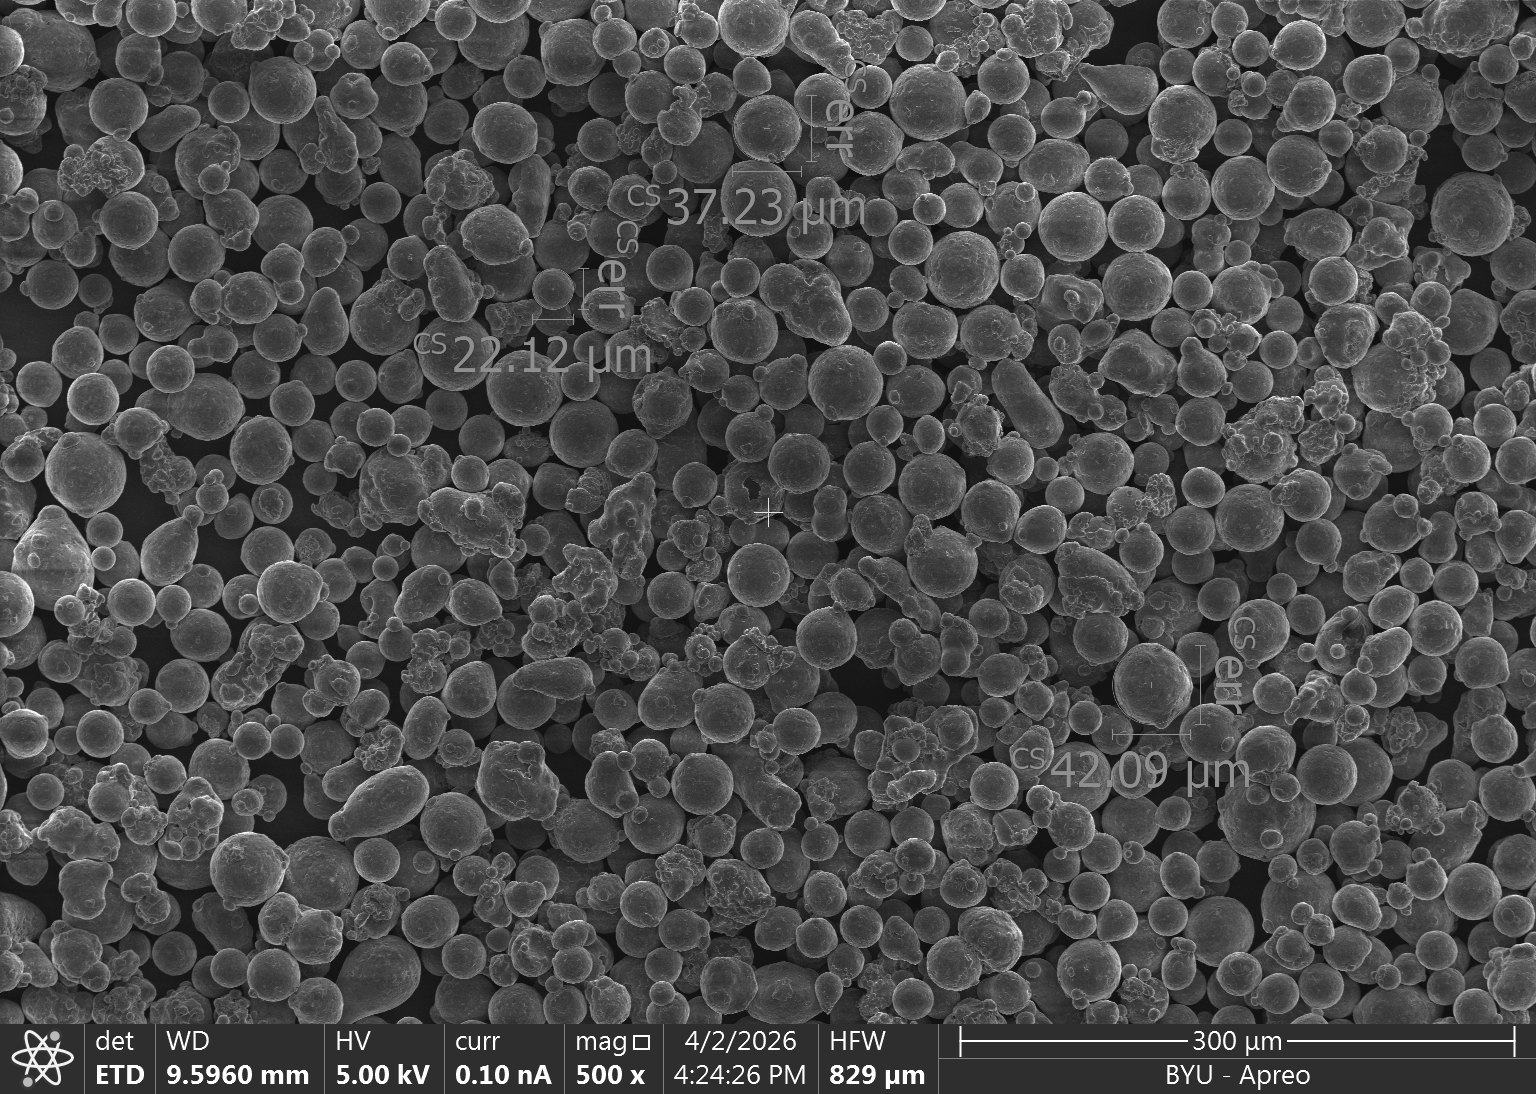
\includegraphics[width=\linewidth]{../figures/sem/AlSi10Mg_slurry_SEM.png}\\[1pt]
    {\scriptsize SEM: stock AlSi10Mg powder (BYU).}
  \end{minipage}\hfill
  \begin{minipage}[t]{0.44\linewidth}
    \centering
    \fbox{\begin{minipage}[c][0.9in][c]{0.92\linewidth}
      \centering\scriptsize
      \textit{Placeholder:}\\
      AMAZEMET-atomized\\ AlSi10Mg+Si+Al-wire\\ blend: SEM + EDS maps\\.
    \end{minipage}}
  \end{minipage}
  \caption{AlSi10Mg baseline and composition-adjustment workflow: (\textit{top})~Thermo-Calc AM~Module prediction for stock AlSi10Mg and a Si-enriched variant; (\textit{bottom-left})~SEM of stock AlSi10Mg feedstock (BYU in-hand); (\textit{bottom-right})~AMAZEMET-atomized AlSi10Mg+Si+Al-wire blend with SEM and EDS (partner run in progress). Illustrates end-to-end CALPHAD\,$\to$\,atomize\,$\to$\,characterize readiness on a familiar baseline alloy.}
  \label{fig:baseline}
\end{wrapfigure}

\flaime{} bridges computation and physical qualification using \bofn{} augmented by an additional mineral-burden
objective~\cite{astudillo_2019_icml,astudillo_2021_21121531}, building on
supply-risk-aware optimization~\cite{mulukutla_2024_ssrn4968}; recent
cost-aware BO advances make AI-guided powder-to-property discovery
tractable~\cite{chawla_2025_arxiv251116930}.

Three lines of preliminary evidence support \flaime{}'s readiness:
(1)~CALPHAD evaluation via Thermo-Calc TCAl10/TCMG6 with Scheil and
AM~Module analysis already identifies printable compositions across the
\elementcount-element palette (Al--Mn--Cr--Zr and Al--Zr initial results
in Fig.~\ref{fig:anchor-calphad});
(2)~an AlSi10Mg baseline exercises the full
design\,$\to$\,atomize\,$\to$\,characterize loop (Fig.~\ref{fig:baseline});
and (3)~in-house pKGFN~\cite{buathong_2023_23110214} benchmarks on
manufacturing-like test networks demonstrate convergence superior to
standard BO baselines (Fig.~\ref{fig:pipeline}).

The Lead PI brings direct SDL experience since 2022---including three
years of technical leadership at the Acceleration Consortium, where he
advanced workflow orchestration and human-in-the-loop SDL
design---and lead-authored the structural-materials section of a
comprehensive SDL review~\cite{tom_2024_acschemr}, the frugal-twin
framework for resource-constrained labs~\cite{lo_2024_d3dd0022}, and a
critical-raw-materials roadmap~\cite{titirici_2022_roadmap}.  Prior
high-dimensional BO work~\cite{baird_2022_commatsci,baird_2023_dib}
directly informs \flaime{}'s search over \subsystemcount{}
sub-systems.  Funded industry partners anchor the pipeline:
\textbf{Valimet} (gas atomization),
\textbf{AMAZEMET} (ultrasonic atomization via rePOWDER), and \textbf{Thermo-Calc AB} (TCAl10/TCMG6 +
AM~Module).  Partner roles are detailed in Methods
(\S\ref{sec:methods}, Activity~2).

% --- 2. Project Objectives (~0.5 page) -------------------------------------
\section{Project Objectives}\pagebudget{0.5}
\label{sec:objectives}

\guidance{FOA: ``Provide a clear and concise statement of the specific
objectives of the proposed project.  Address how the objectives align
with the chosen focus topic and lead to an AI advantage.''  Keep
objectives quantitative, measurable, and few (3--5).}

\guidance{COMMERCIALIZATION (Review Criterion 4, FOA p.85): ``Does the
application articulate a credible strategy for technology transfer
and/or commercialization beyond the project's duration?''  Since AMMTO
is an applied technology office, include at least one objective or
sentence addressing technology transfer path (e.g., software licensing,
industry partnership, standards body engagement).}

\noindent\textbf{Goal.} Discover novel, high-performing, critical-mineral-lean
LPBF aluminum alloys for structural applications and demonstrate a
measurable AI advantage through established
metrics~\cite{tom_2024_acschemr}---specifically, AI acceleration
factor, discovery yield, and mineral-burden
reduction---advancing the dual Topic~3B
mandate of AI-enabled materials discovery \emph{and} reduced demand
for critical minerals.

\begin{enumerate}[label=\textbf{O\arabic*.},leftmargin=2em]
  \item Demonstrate a closed-loop BOFN/pKGFN platform for AI-guided,
        cost-aware alloy exploration across the full powder-to-property pipeline.
  \item Evaluate \subsystemcount{} element combinations ($k=2$--$8$ from a
        \elementcount-element palette) and 100--200 compositions within selected
        sub-systems via CALPHAD with an integrated mineral-burden objective.
  \item Validate 100--200 compositions experimentally through the
        minimum-viable-specimen (MVS) pipeline over a 9-month Phase~I
        (throughput derivation in App.~\ref{app:facilities}).
  \item Achieve overall discovery yield $\geq$3\%---i.e., at least 3--6
        high-performing alloys meeting family-specific mechanical targets
        (e.g., Al-Mn-Cr-Zr: YS$\geq$250\,MPa, EL$\geq$5\%;
        Al-Zr: YS$\geq$200\,MPa, EL$\geq$8\%, with elevated-temperature
        retention) \emph{and} mineral-burden reduction $\geq$40\% vs.\
        Scalmalloy; complementary metric:
        $\geq$20\% Tier~1 pass rate among $\geq$20 fully tested compositions.
  \item Demonstrate AI acceleration factor~\cite{tom_2024_acschemr} $\geq$3$\times$ vs.\ a
        pre-registered random baseline~\cite{sabanzagil_2025_s4358802}, with
        bootstrap confidence intervals across $\geq$20 seeds.
\end{enumerate}

\noindent Collectively, fulfillment of these objectives demonstrate that a
software-orchestrated, AI-guided closed-loop platform can
simultaneously accelerate alloy discovery \emph{and} reduce critical
mineral dependence---the dual mandate of Topic~3B. Phase~I focuses on
Al alloys processed by LPBF, with Cu-Cr-Zr as a stretch demonstration.
The \elementcount-element palette (Al~+~\elementlisttex{}) spans 0\%
to 100\% USGS import reliance, ensuring the mineral-burden objective
produces genuine supply-risk tradeoffs.

\flaime{} advances from TRL~2 to TRL~4 at Phase~I exit (closed-loop
validated on real Al alloys)~\cite{tom_2024_acschemr}.  Phase~II
extends to higher-temperature structural materials (Cu-Cr-Zr, 316H) via
transfer learning and full-size
testing~\cite{wang_2020_17452759,karnati_2022_mpc20210136},
expands atomization to plasma-based ultrasonic methods (AMAZEMET
partnership), and replaces each Phase~I human handoff with a robotic
endpoint.  Methodologically, Phase~II will explore incorporation of LLM
priors into the pKGFN framework---building on the LILO
(Language-in-the-Loop Optimization)
approach---as a stretch goal; robust benchmarking of such hybrid
LLM--BO methods remains an open challenge~\cite{liu_2024_llambo}.

\textbf{Technology transfer and commercialization.}  All \flaime{}
software will be released open-source under a permissive license,
building on the Lead PI's extensive track record in open-source
scientific software (17K+ code artifacts, creator of the
\texttt{awesome-self-driving-labs} community-curated resource list).
The BO pipeline modules will be contributed as
BoTorch~\cite{balandat_2019_19100640} tutorials---supported by a
letter of collaboration from Meta---and integrated into
Honegumi~\cite{baird_2025_honegumi}, a widely used materials
informatics template engine (24K~page views, 6K~unique visitors across
10~countries since April~2024).  Discovered alloy compositions will be
published openly rather than licensed: Scalmalloy, the highest-impact AM
aluminum alloy, is patented but achieved broad commercial
adoption primarily through standardization and industry partnerships
rather than exclusive licensing restrictions.  To accelerate industry
validation, \texttt{[TBD\_N\_UNIV]} universities, \texttt{[TBD\_N\_LAB]}
national laboratories, and \texttt{[TBD\_N\_COMPANY]} companies
have written letters of collaboration expressing intent to print with
3--6 validated compositions scaled up to gas atomization at varying
particle size distributions (\texttt{[TBD\_N\_LPBF]}~LPBF,
\texttt{[TBD\_N\_DED]}~DED, \texttt{[TBD\_N\_BJ]}~Binder Jet) and
return at least one sample with related metadata (e.g., scan settings).
This multi-site validation network, combined with FAIR
data practices, open software, and a path toward adoption by major
powder manufacturers through composition disclosure and standardization
engagement, ensures that \flaime{}'s discoveries
propagate rapidly to the broader AM community.

% --- 3. Proposed Research and Methods (~1.5 pages) --------------------------
\section{Proposed Research and Methods}\pagebudget{1.5}
\label{sec:methods}

\guidance{FOA: ``Provide a clear research plan for a 9-month project
and describe the proposed activities and methods.  Include enough
technical details to evaluate the impact of the proposed activity.  For
each activity, indicate the responsibility of the key investigator(s)
and the associated budget.  If building on existing DOE-funded work,
describe how this is distinct.''}

\instruct{This is the center of gravity.  Must cover:
(1) AI framework (\bofn{} DAG or equivalent),
(2) experimental pipeline (powder $\to$ print $\to$ test),
(3) closed-loop integration,
(4) qualification-relevant data generation.
Include a system architecture figure if it fits within the 5-page
limit --- otherwise move it to an appendix reference or describe
textually.  Tables and figures count against the limit, so use them
very selectively.}

\guidance{PHASE I $\to$ PHASE II (FOA p.57): Only ``a small fraction''
of Phase I teams will advance to Phase II.  Frame Phase I as
demonstrating readiness for 3x--5x scale-up.  Reference how the
platform generalizes from the demonstration alloy system to AMMTO's
core materials portfolio (e.g., 316H, IN718, Hastelloy N) in Phase II
(\$6M--\$15M, 3 years).}

\guidance{FULL PIPELINE DESCRIPTION (FOA p.70): ``Applications should
describe the full pipeline of data generation and curation; experiments
and observation, AI model training, fine tuning, and inferencing; and
integration, using agentic techniques or otherwise, into a capability
of use for science or engineering.''  Ensure all pipeline stages are
explicitly addressed.}

\guidance{TEAM COORDINATION (Review Criterion 3, FOA p.84): ``To what
extent does the application demonstrate a clear, well-coordinated
collaboration among partnering institutions, with appropriately balanced
responsibilities, synergistic contributions, and clearly defined roles
for each team member?''  Address communication cadence, data handoff
protocols, and decision-making structure.}

\textbf{Activity~1: AI-Guided Computational Exploration}
(\emph{PI, BYU; {$\sim$}\$200K}).
%
The \flaime{} optimizer is a Bayesian Optimization over Function
Networks (\bofn{}) directed acyclic graph
(DAG; Fig.~\ref{fig:pipeline},
right)~\cite{sundar_2025_s4357802,paramore_2025_jactamat} covering
Thermo-Calc AM~Module simulation, powder, LPBF, and mechanical-response nodes.
The \emph{partial} Knowledge Gradient for Function
Networks (pKGFN)~\cite{buathong_2023_23110214,buathong_2025_25061145}
is the acquisition function that selects which node and inputs to
evaluate next in a cost-aware manner: ``partial'' because not every
node is evaluated at each iteration (e.g., a Thermo-Calc AM~Module
query can be run without triggering an expensive tensile test),
``knowledge gradient'' because the decision maximizes the expected
improvement in the global objective per unit cost across fidelities
ranging from Thermo-Calc AM~Module simulation to full
powder dosing, atomization, LPBF printing, and tensile testing, and
``network'' because the DAG structure---where
each node's output feeds downstream nodes---is
exploited to propagate information efficiently.
A mineral-burden
node ($\mathrm{MBS}=\sum_i w_i\,x_i$; analytical, noise-free)
incorporating USGS import-reliance weights, Graedel supply-risk
indices~\cite{graedel_2012_es203534}, and ESSENZ characterization
factors~\cite{cimprich_2019_jiec1286} enables
multi-objective strength \emph{and} supply-risk optimization.
Preliminary pKGFN convergence
(Fig.~\ref{fig:pipeline}, left) and active CALPHAD evaluation on BYU
HPC confirm readiness.  LLM-augmented initialization
via LLAMBO~\cite{liu_2024_llambo} provides informed seeds
(${>}16\%$ efficiency gain in benchmarks); LLAMBO supplies warm-start
prior means for the GP surrogate, not metallurgy-specific reasoning.

\begin{wrapfigure}{r}{0.48\textwidth}
  \centering
  \vspace{-\intextsep}
  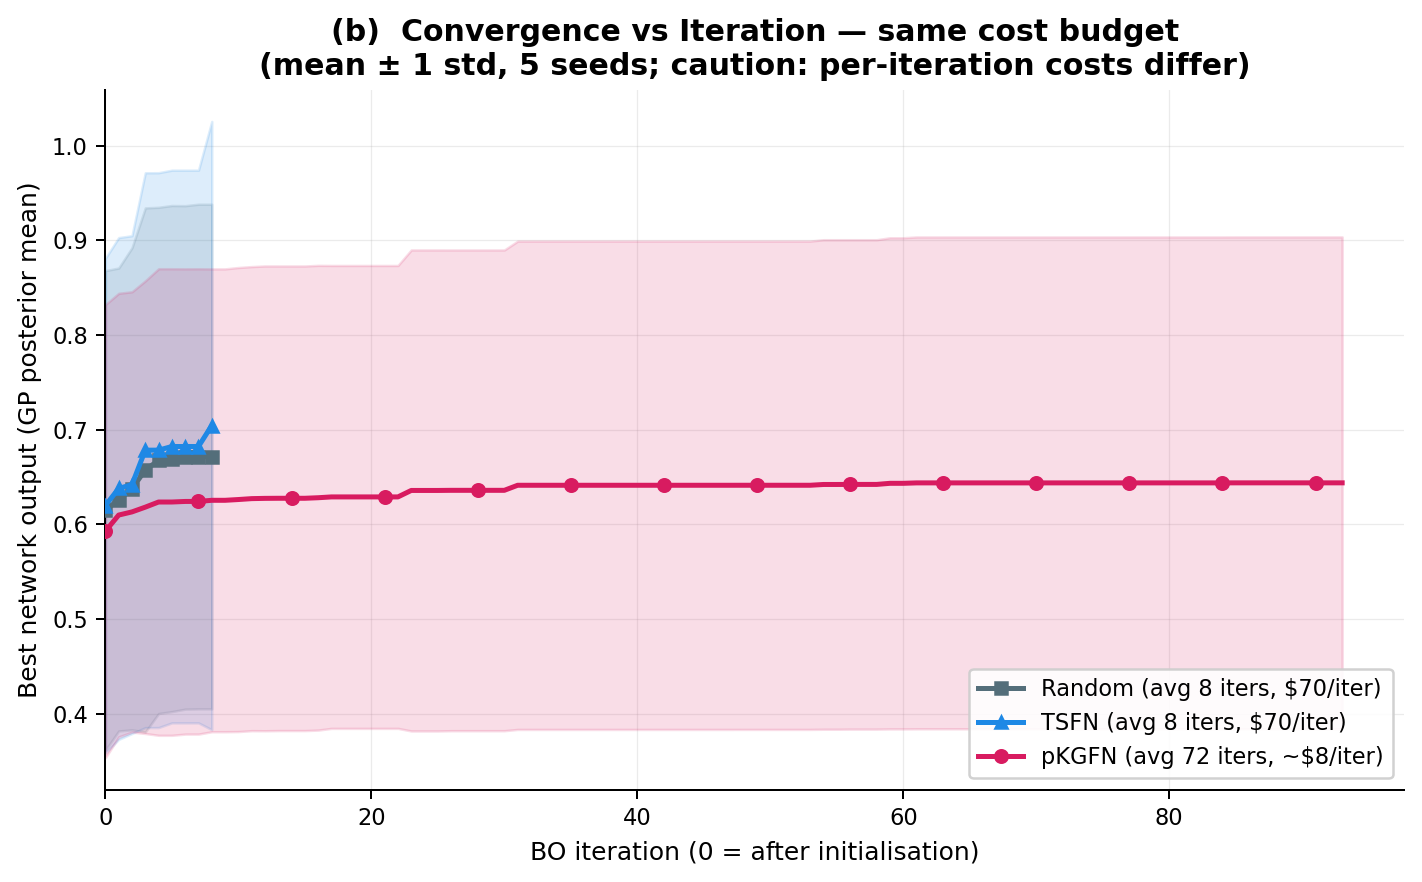
\includegraphics[width=\linewidth]{../benchmarks/figures/pkgfn_convergence.png}\\[3pt]
  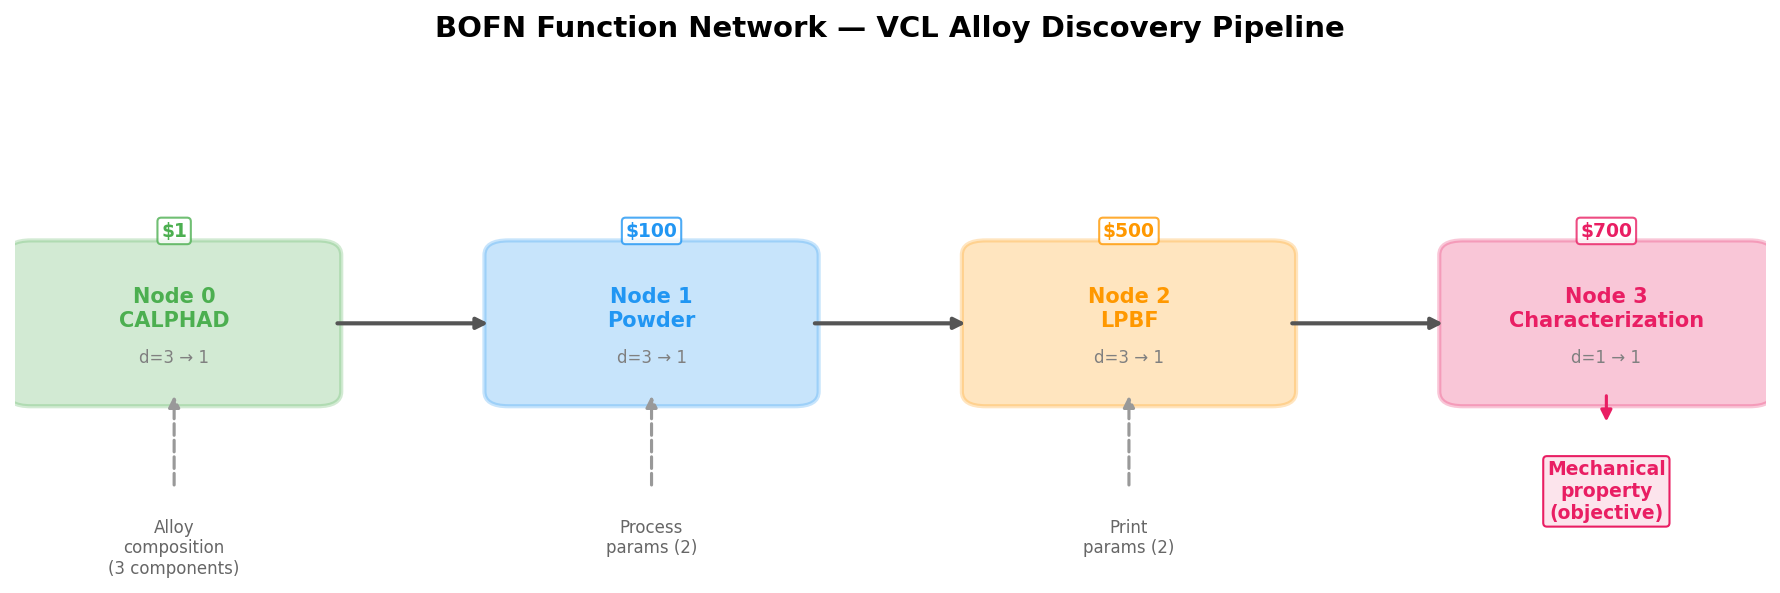
\includegraphics[width=\linewidth]{../benchmarks/figures/bofn_dag.png}
  \caption{\textit{Top:} pKGFN convergence on a manufacturing benchmark vs.\ standard BO baselines. \textit{Bottom:} \bofn{} DAG for the \flaime{} pipeline; pKGFN selects the most cost-informative next experiment across CALPHAD, atomization, LPBF, and testing nodes.}
  \label{fig:pipeline}
\end{wrapfigure}

\textbf{Asynchronous, Cost-Aware Exploration.}
pKGFN jointly optimizes over composition, atomization, and print
parameters---\emph{not} as a sequential screen-and-filter funnel, but
as a single adaptive BO loop spanning all
$\sum_{k=2}^{8}\binom{\elementcount}{k}=\subsystemcount{}$
sub-systems (${\sim}$\num{119000000} compositions at 1\,at.\%,
Al\,$\geq$\,85\,at.\%), a novel NChooseK
problem~\cite{mamun_2025_ada47d,daulton_2022_22101019}.
Asynchronous BO treats pending HPC jobs as fantasy
samples (surrogate predictions for pending points temporarily added to
the model to avoid redundant suggestions---a standard batch-conditioning
technique).  Sobol quasi-random sequences provide initial
space-filling designs, chosen over Latin Hypercube Sampling for their
ability to incrementally add new points without losing space-filling
properties.
%
Rapid \texttt{pycalphad}~\cite{otis_2024_97810035} evaluations
compute phase fractions,
Scheil curves~\cite{bocklund_2020_20011161}, CSI, and mineral-burden
scores; these serve as \emph{contextual features}---assigned learnable
weights in the GP surrogate that can be down-weighted or removed if
correlation with downstream nodes is low---rather than as DAG nodes.
%
\emph{Fidelity~2} (TC-Python + TCAl10; {$\sim$}1--5\,CPU-min/eval):
Scheil with back-diffusion and TC-PRISMA
precipitation kinetics for targeted sub-systems.
%
\emph{Fidelity~3} (Thermo-Calc AM~Module, {$\sim$}0.5--2\,CPU-hr/eval):
printability maps, melt-pool geometry, and Scheil at LPBF cooling rates
($10^{4}$--$10^{6}$~K/s)---many of these parameters map directly to
tunable settings on the Aconity MIDI's open-parameter
architecture---inform candidate viability before
atomization; FLAIME prints reciprocally calibrate the AM~Module's
aluminum absorptivity (Appendix~2), and AM~Module simulations can be
re-run post-improvement and replaced into the surrogate to improve the campaign itself.
%
For expensive prediction nodes in 6+ component spaces,
SAASBO~\cite{eriksson_2021_21030034} identifies sparse relevant
subspaces (scaling as $n^{3}$ in data points, limiting to hundreds of
evaluations---appropriate for the experimental budget); SVDKL
deep-kernel GPs~\cite{sabanzagil_2025_s4358802}
handle phase-boundary non-stationarity.
%
Al--Mn--Cr--Zr and Al--Zr serve as
initial focus systems (Fig.~\ref{fig:anchor-calphad}): Al--Mn--Cr--Zr
is one of the most promising lightweight high-strength LPBF systems in
the recent literature~\cite{thapliyal_2020_jmtla201}; Al--Zr offers
L1$_{2}$ precipitate strengthening with excellent thermal stability.
Both receive experimental validation early in Phase~I to establish
surrogate calibration, but pKGFN routes subsequent evaluations across
the full search space based on cost-aware expected information gain, not
predetermined sub-systems.

\begin{wrapfigure}{l}{0.30\textwidth}
  \centering
  \vspace{-\intextsep}
  \fbox{\begin{minipage}[c][0.9in][c]{0.95\linewidth}
    \centering\scriptsize
    \textit{Placeholder:} \texttt{example-image-a} (Al--Mn--Cr--Zr and Al--Zr CALPHAD from TCAl10/AM~Module).
  \end{minipage}}
  \caption{Initial focus sub-system CALPHAD output for Al--Mn--Cr--Zr and Al--Zr using TCAl10/AM~Module.}
  \label{fig:anchor-calphad}
\end{wrapfigure}

\textbf{Activity~2: Experimental Validation Pipeline}
(\emph{PI + partners; BYU {$\sim$}\$300K + Valimet + AMAZEMET}).
%
Powder feedstocks are produced via ultrasonic atomization (AMAZEMET
rePOWDER with induction crucible module, BYU, en-route from Poland as of 2026-04-24) for rapid composition
iteration---mixtures of elemental powders are dosed at 0.1\,mg
resolution (typical 100\,g batches) into machined high-purity aluminum
crucibles (jointly serving as the bulk Al contribution, the ``dispense vial'', and a compaction die, see Appendix 2), providing high compositional design freedom---and gas
atomization (Valimet partnership) for a subset of production-scale lots.
SEM/EDS of atomized
powders (Fig.~\ref{fig:baseline}) targets ${\leq}2$\,wt\% composition
deviation from design; AMAZEMET verification runs on the AlSi10Mg+Si+Al-wire
blend have been atomized in advance through pre-collaboration with AMAZEMET.
LPBF printing is performed at the University of Utah (Prof.\ Ashley
Spear's lab, Aconity MIDI; 3D~Powder Tech backup).  A minimum-viable-specimen (MVS)
progression manages throughput on a partial-evaluation, cost-aware basis:
single tracks (one BOFN node) $\to$ thin-wall
structures for crack susceptibility screening (one BOFN node) $\to$
$5{\times}5{\times}5$\,mm density cubes (${\geq}99$\% relative density
gate; one BOFN node) $\to$ ASTM~E8/E8M tensile bars
(Fig.~\ref{fig:composite}, Appendix~2),
where each of these four AM test structure nodes require completion of its predecessor test structures but
any stage can be early-stopped without proceeding further.
An initial specific composition
(Al-\texttt{[TBD]}at.\%\,Mn-\texttt{[TBD]}at.\%\,Cr-\texttt{[TBD]}at.\%\,Zr)
has been sent to Thermo-Calc for AM~Module evaluation.

Sub-size ASTM~E8/E8M (sub-size, 100 mm length instead of 200 mm) specimens are standard in LPBF
screening~\cite{paraschiv_2023_ma16144930,wang_2020_17452759} (YS/UTS
within ${\sim}5$\%~\cite{paraschiv_2023_ma16144930}; elongation per
ASTM~E8/E8M~\cite{astm_2024_e8e8m}).  Tiered screening routes
${\sim}50$--${\sim}200$ compositions through tensile testing (conservative
lower bound 50; upper bound set by the rate of success through the
atomize--print--density-gate pipeline) and ${\sim}150$--${\sim}450$ through
hardness/density; Preliminary results involving printing AlSi10Mg and performing tensile tests have been carried out (Fig.~\ref{fig:tensile}).
  All compositions undergo elevated-temperature
testing at three temperatures as additional objectives, validating L1$_2$
stability for DOE thermal applications with similar or greater performance and lower critical mineral usage than the incumbent Al--Zr.
Authoritative elemental composition verification uses
ICP-MS (BYU Spectroscopic Facility, Agilent 8900 ICP-MS/MS)
complementing semi-quantitative SEM/EDS.

\begin{wrapfigure}{r}{0.36\textwidth}
  \centering
  \vspace{-\intextsep}
  \fbox{\begin{minipage}[c][0.95in][c]{0.95\linewidth}
    \centering\scriptsize
    Placeholder:\\
    AlSi10Mg tensile curves + YS/UTS/EL bars
  \end{minipage}}
  \caption{AlSi10Mg tensile data (stress--strain, YS/UTS/EL; ASTM~E8, U.Utah).}
  \label{fig:tensile}
\end{wrapfigure}

\textbf{Activity~3: Closed-Loop Integration, Dissemination \&
Qualification} (\emph{PI, BYU; {$\sim$}\$100K}).
%
The pKGFN engine orchestrates autonomous cycles: GP surrogates retrain
after each batch and select next compositions and parameters;
software-dispatched SOPs map human handoffs 1:1 to Phase~II robotic
points, requiring robotic implementation while keeping the workflow
redesign and orchestration infrastructure intact (i.e.,
software-orchestrated human-in-the-loop significantly reduces the
technical debt accrued when shifting to software-orchestrated robotic
workflows).  ISO~52902 benchmark geometries are printed as a BOFN node
throughout the campaign (not only at project end), providing
qualification-relevant artifacts with digital-thread provenance
(composition, CALPHAD, powder, LPBF parameters, ASTM~E8, BOFN).
Data capture uses a document-based cloud database (MongoDB) that can
evolve into a relational schema once the workflow stabilizes, with a
graph database (Phase~II) for full provenance queries.
Plug-and-play tutorials integrate into Honegumi~\cite{baird_2025_honegumi}
and BoTorch~\cite{balandat_2019_19100640} (Meta letter of collaboration);
the PI's POSE, Acceleration Consortium, and GCMAC record ensures
\flaime{} outputs become community tools shared via Genesis Mission
platform and open repositories.

\textbf{Project Management \& Risk Mitigation.}
Weekly PI--partner calls and monthly reviews maintain alignment; a
FAIR-compliant database is the single source of truth.  Ten
undergraduates operate in shifts for six-day/week throughput (${\geq}8$
compositions/month), each assigned a specific stage under PI/MS oversight.
Key fallbacks: (i) low atomization yield $\to$ Valimet gas-atomization;
(ii) modest \bofn{} advantage $\to$ honest reporting via pre-registered
time-ledger; (iii) LPBF disruption $\to$ 3D~Powder Tech;
(iv) characterization bottleneck $\to$ tiered screening (${\sim}50$
tensile~+~${\sim}150$ density/hardness).

\textbf{Relationship to Prior Work.}
\flaime{} builds on the PI's Honegumi SDL infrastructure and Fehrmann
Materials ML-guided alloy contract, but represents fundamentally new
closed-loop integration of composition discovery with AM
qualification---no prior DOE funding supports this work.

% --- 4. Milestones in the Nine Months (~1 page) ----------------------------
\section{Milestones in the Nine Months}\pagebudget{1}
\label{sec:milestones}

\guidance{FOA: ``Provide a list of clearly defined and measurable
milestones of the project.''  These should be concrete deliverables, not
activities.  Include Go/No-Go decision gates.}

\begin{table}[H]
\centering\small
\caption{Phase~I milestones and deliverables (9~months).}
\label{tab:milestones}
\begin{tabularx}{\textwidth}{clX}
\toprule
\textbf{Mo.} & \textbf{ID} & \textbf{Milestone / Deliverable} \\
\midrule
1 & M1 & BOFN DAG deployed; multi-fidelity CALPHAD evaluation (pycalphad, TCAl10, AM~Module) operational on BYU HPC; Fidelity~1 element-combination assessment (\subsystemcount{} sub-systems) complete; Fidelity~2/3 evaluation of targeted sub-systems initiated; Al--Mn--Cr--Zr and Al--Zr initial focus compositions selected for experimental validation \\
2 & M2 & First atomized powder batches characterized (PSD, SEM/EDS, flowability); pre-registered 5-baseline benchmark design frozen; formal provenance schema deployed \\
3 & M3/G1 & \textbf{Go/No-Go G1:} $\geq$50 compositions screened computationally; GP surrogate RMSE $<$ pre-registered threshold on nested CV. \textit{If fail: retrain surrogate with augmented CALPHAD data; extend G1 by 1~month.} \\
5 & M4/G2 & \textbf{Go/No-Go G2:} $\geq$1 complete AI-orchestrated CALPHAD$\to$atomization$\to$LPBF$\to$tensile$\to$BOFN cycle demonstrated end-to-end (software-dispatched, human-executed); $\geq$2 compositions at $\geq$99.0\% relative density. \textit{If fail: decouple pipeline; run stages independently with manual scheduling.} \\
7 & M5/G3 & \textbf{Go/No-Go G3:} $\geq$1 alloy meeting family-specific thresholds (Al-Mn-Cr-Zr: YS$\geq$250~MPa, EL$\geq$5\%; Al-Zr: YS$\geq$200~MPa, EL$\geq$8\%) or $\geq$1 alloy from an AI-discovered sub-system meeting equivalent thresholds, with SRI$_\text{mean}$ $\geq$25\% below Scalmalloy; ASTM~E8 sub-size data with $\geq$3 replicates. \textit{If fail: pivot to strongest partial-pass composition; intensify BOFN exploitation.} \\
9 & M6 & Final deliverables: digital thread ($\geq$85\% completeness with supply-risk metadata); Critical Mineral Demand Reduction Index (CMDRI) calculation vs.\ Scalmalloy ($\geq$40\% reduction target) and AlSi10Mg; pre-registered AI benchmark report (AF, win rate, bootstrap CI); Phase~II readiness assessment \\
\midrule
\multicolumn{3}{l}{\textit{Stretch (non-gated):}} \\
9 & S1 & Cu-Cr-Zr feasibility: $\geq$1 atomized Cu-Cr-Zr powder batch with PSD within LPBF spec; CALPHAD surrogate trained; Phase~II targets: YS$\geq$200~MPa, $\geq$50\% IACS \\
\bottomrule
\end{tabularx}
\end{table}

\instruct{Milestones must be clearly defined and measurable --- not just
``continue work on X.''  Each Go/No-Go gate should have a quantitative
pass/fail criterion.  Example: G1 = AI model trained on $\geq$50
compositions with RMSE $<$ threshold; G2 = closed-loop cycle
demonstrated end-to-end; G3 = $\geq$1 alloy meeting target properties.}

\guidance{6-MONTH DOE REVIEW POINT (FOA p.61): ``go/no go evaluation at
6 months.''  Structure the milestone table around this checkpoint --- the
month 5--7 Go/No-Go gates are the primary decision point for DOE
program managers.  The final 9-month milestones confirm completion but
the 6-month review determines continuation.}

% --- 5. Data Sources and Models (~0.5 page) --------------------------------
\section{Data Sources and Models}\pagebudget{0.5}
\label{sec:data}

\guidance{FOA: ``Describe which existing or new data sources will be
used.  Address your team's access to the data.  If applicable, indicate
which AI models or frameworks will be used.  Do NOT include computing
resource descriptions here --- that goes in Appendix 2 (Facilities).''}

\textbf{Data sources.}
CALPHAD: Thermo-Calc TCAl10 (Al) and TCMG6 (Mg) via the TC-Python API
under BYU's HPC license (Thermo-Calc commitment letter, Appendix~7).
DFT formation energies from Materials
Project~\cite{jain_2016_14944683} and AFLOW~\cite{oses_2018_18030503}
augment surrogate inputs via Matminer~\cite{ward_2018_jcommats}.
Experimental benchmarks: MMPDS, Knovel (Utah institutional access), and
the ASM Alloy Center Database.
Supply-risk scoring uses USGS Mineral Commodity
Summaries~\cite{usgs_mcs_2024} and the DOE Critical Materials
Assessment~\cite{bauer_2023_1998242} for element-level import-reliance
and criticality; Mulukutla et al.~\cite{mulukutla_2024_ssrn4968}
precedents integration of these metrics into Bayesian optimization.
All \flaime{}-generated data will be published on Zenodo/Figshare with
persistent DOIs; the PI's widely reused MPTS-52 dataset evidences this
open-data commitment.

\textbf{AI models.}
Bayesian Optimization over Function Networks (\bofn{}) with the partial
Knowledge Gradient (pKGFN) acquisition drives cost-aware selection atop
GPyTorch/BoTorch GP surrogates~\cite{balandat_2019_19100640}.
\bofn{}/pKGFN will be released as open-source Python packages with
Honegumi tutorials, integrated into the BoTorch ecosystem (Meta letter
of collaboration, Appendix~7).

\textbf{Genesis Mission integration.}
\flaime{} is designed for American Science Cloud (AmSC) hosting of its
digital thread, alloy database, and \bofn{}/pKGFN models as a
``plug-and-play'' capability per the GM framework, with parallel
Zenodo/Figshare deposit (FAIR, persistent DOIs).  \flaime{}
bidirectionally leverages other GM teams' characterization and
benchmark data to accelerate CALPHAD surrogate training
(Appendix~4~DMSP).

% --- 6. Decision Gate Metrics (~0.5 page) -----------------------------------
\section{Decision Gate Metrics}\pagebudget{0.5}
\label{sec:gates}

\guidance{FOA: ``Provide specific metrics that can be used for the
evaluation of Phase I go/no go decision.  DOE encourages the development
of metrics to identify AI advantage.  One such metric could include
scaling behavior which shows increasing performance as additional data,
computing, and/or other resources are applied.  Quantitative statements
enabling transformative science and engineering through AI are
preferred.''}

\instruct{Key metrics to define: (1) AI advantage metric (e.g.,
compositions screened per unit time vs.\ conventional), (2) scaling
behavior (does performance improve with more data/compute?), (3)
qualification-relevant metric (how much of the traditional qualification
process is compressed?).  All metrics must be quantitative.}

\guidance{SCALABILITY (Review Criterion 2, FOA p.84): ``Does the
application address potential scalability issues?''  Include at least
one metric demonstrating scaling behavior --- e.g., compositions
screened per week as dataset grows, or model accuracy as function of
training data volume.  AMMTO values paths from lab-scale to
production-scale.}

\guidance{AI ADVANTAGE --- define precisely what ``AI advantage'' means
for this project: (1)~10x faster screening (5 days/composition vs.\
8--32 weeks conventional), (2)~autonomous experimental campaigns that
reduce human labor per composition, (3)~compressed qualification
timelines via digital thread.  The FOA uses ``AI advantage'' as a
central evaluation concept; your Decision Gate Metrics must quantify it.}

Table~\ref{tab:gates} defines Phase~I go/no-go metrics.

\begin{table}[H]
\centering\small
\caption{Phase~I Decision Gate Metrics.}
\label{tab:gates}
\begin{tabularx}{\textwidth}{lXl}
\toprule
\textbf{Metric} & \textbf{Definition} & \textbf{Phase~I target} \\
\midrule
AI Acceleration Factor (AF) &
$\mathrm{AF}(y) = n_{\mathrm{baseline}} / n_{\mathrm{BOFN}}$:
iteration reduction \bofn{} achieves vs.\ four pre-registered
baselines---random~(B1), expert DOE~(B2), standard BO~(B3), \bofn{}
ablation without mineral-burden~(B4)---with $\geq$20 replicate seeds,
bootstrap CI, and win-rate reporting (SDL cross-study median
$\sim$6$\times$~\cite{sabanzagil_2025_s4358802}). &
$\geq$3$\times$ vs.\ random \\
\addlinespace
Discovery Yield &
Fraction of BOFN-proposed compositions satisfying all family-specific
mechanical thresholds (e.g., Al-Mn-Cr-Zr: YS\,$\geq$\,250\,MPa,
EL\,$\geq$\,5\%; ASTM~E8 sub-size) \emph{and} supply-risk reduction
vs.\ Scalmalloy.  The \elementcount-element palette spans 0\% (Fe) to
100\% (Sc) USGS import reliance, ensuring genuine tradeoffs. &
$\geq$\,3\% \\
\addlinespace
Mineral-Burden Reduction &
Weighted critical-mineral content (wt\,\%) of best-performing
\flaime{} alloy vs.\ Scalmalloy incumbent (Al-Mg-Sc-Zr). &
$\geq$\,40\% \\
\bottomrule
\end{tabularx}
\end{table}

\textbf{Scaling behavior.}
BOFN surrogate accuracy (GP RMSE on hold-out compositions) and
acquisition efficiency (AF metric) improve monotonically with
accumulated CALPHAD-screened and experimental data.  Phase~I will
quantify this via learning curves: GP RMSE and AF will be plotted
against dataset size at regular intervals (every 25 compositions),
producing a scaling curve that demonstrates diminishing marginal
regret per additional evaluation---a hallmark of well-calibrated
surrogate-driven optimization.  We expect GP RMSE to decrease by
${\geq}50$\% from the initial Sobol-seeded model to the final
Phase~I surrogate.

\textbf{AI Tool Disclosure.}
Edison Scientific supported literature search and proposal planning (${\sim}$120 queries).  GitHub Copilot (Claude Opus 4.6) assisted code development and drafting.  All AI-generated content was reviewed, validated, and revised by the proposed researchers.

% ============================================================================
%  APPENDIX 1: BIBLIOGRAPHY & REFERENCES CITED
%  (Does NOT count against 5-page narrative limit)
% ============================================================================
\newpage
\section*{Appendix 1: Bibliography \& References Cited}
\label{app:references}

\required{FOA \S IV.C: ``Provide a bibliography of any references cited
in the Project Narrative.  Each reference must include the names of all
authors (in the same sequence in which they appear in the publication),
the article and journal title, book title, volume number, page numbers,
and year of publication.'' No page limit for this appendix.}

% Include refs that appear in the bibliography but are not yet \cite'd inline.
% These were in the original hand-written list; add inline \cite's as the
% narrative is expanded.
\nocite{abolhasani_2023_s4416002}  % [old 1]  Abolhasani & Kumacheva, Nat. Synth. 2023
\nocite{stach_2021_jmatt202}       % [old 2]  Stach et al., Matter 2021
\nocite{buathong_2023_23110214}    % [old 6]  Buathong et al., partial evaluations 2023
\nocite{khatamsaz_2023_s4152402}   % [old 7]  Khatamsaz et al., npj Comp. Mat. 2023
\nocite{liang_2025_sciadvad}       % [old 8]  Liang et al., Science Advances 2025
\nocite{bukkapatnam_2023_24725854} % [old 9]  Bukkapatnam, IISE Trans. 2023
\nocite{isoastm_52902_2023}        % [old 16] ISO/ASTM 52902:2023
\nocite{isoastm_52907_2019}        % [old 18] ISO/ASTM 52907:2019

\instruct{Must cite inline (currently only \textbackslash nocite'd):
Abolhasani \& Kumacheva 2023 (Nat.\ Synth.),
Stach et al.\ 2021 (Matter),
Khatamsaz et al.\ 2023 (npj Comput.\ Mater.),
Liang et al.\ 2025 (Sci.\ Adv.).}

\renewcommand{\bibsection}{}% suppress auto-generated "References" heading
\bibliographystyle{unsrtnat}
\bibliography{edison-references}

% ============================================================================
%  APPENDIX 2: FACILITIES & OTHER RESOURCES
%  (0.5 page max; does NOT count against narrative limit)
% ============================================================================
\newpage
\section*{Appendix 2: Facilities \& Other Resources}
\label{app:facilities}

\required{FOA \S IV.C: ``Identify the resources and/or facilities to be
used. If appropriate, indicate their capacities, pertinent capabilities,
relative proximity, and extent of availability to the project. Describe
only those resources that are directly applicable to the proposed work.
Describe the computing, networking, and data resources required.''
Maximum 0.5 page.}

\instruct{Describe: (1) BYU lab --- atomizer, SEM/EDS, tensile tester;
(2) partner LPBF access --- machine specs, access agreement; (3) national
lab facilities if applicable; (4) computing resources (cluster, cloud,
potential DOE HPC allocation).  Frame as leveraging existing DOE-funded
infrastructure where applicable.  If using experimental user facilities
at other institutions, include a document from the facility manager
confirming access.}

\note{FOA notes that DOE computing resources may be available to
selected awardees (FOA \S IV.C, Appendix 2 guidance).  If planning
to request DOE HPC allocations, mention this here.}

\textbf{BYU Materials Discovery Laboratory (Lead Institution).}
The PI's Vertical Cloud Lab (\texttt{[TBD\_SQFT]} sq.\ ft.\ non-shared
lab space; department chair letter confirms allocation and capacity for
Phase~II hardware expansion)
in the Department of Mechanical Engineering houses
an \textbf{AMAZEMET rePOWDER ultrasonic atomizer with induction crucible
module} (scheduled delivery April~30, 2026;
week-long training scheduled), with the dedicated powder metallurgy lab space
nearly fully prepared: canopy hood, industrial dehumidifier, fume hood, dry
powder storage, electrical, gas, air, and chilled water infrastructure installed
in close collaboration with EH\&S and the Engineering Lab Supervisor.
The rePOWDER system accepts mixtures of elemental powders packed into
machined high-purity aluminum crucibles (serving as both vial replacement and
compaction chamber with press-fit lid), providing high compositional design
freedom; the BYU Prototyping Lab is well equipped for machining these
crucibles.  Batch
turnaround is 1--3 compositions per day (per Gantt chart, Appendix~2).
Powder characterization is
performed on-site via the \textbf{BYU Microscopy Center}
(\url{https://microscopy.byu.edu}); several undergraduate researchers are
already trained on SEM.
The powder metallurgy and adjacent Microscopy Center
labs are connected directly by a door with no public access, making the
layout amenable to integration into robotic sample transfer workflows
in Phase~II without the safety and administrative challenges of
public-corridor traversal.
Instruments have high availability, though are not dedicated
exclusively to this project.
The \textbf{BYU Prototyping Lab} (machine shop;
\url{https://capstone.byu.edu/physical-prototyping-resources}) provides CNC
machining, lathe, and mill services for specimen preparation, with a local
\textbf{wire EDM} service in Provo available for precision sectioning (PI has
prior experience); EDM turnaround times are not guaranteed.

\textbf{Partner LPBF Printing Access.}
Laser powder bed fusion capability is provided through \textbf{Prof.\ Ashley
Spear's laboratory at the University of Utah}, which operates an
\textbf{Aconity MIDI} system (170\,mm \textsf{\O} build plate, open-parameter
architecture, 200--1000\,W fiber laser) ideally suited for rapid alloy screening.
Preliminary AlSi10Mg tensile specimens have been printed for baseline validation
(letter of collaboration).
\textbf{3D Powder Tech} provides backup LPBF capacity (letter of collaboration),
ensuring uninterrupted printing throughput.

\textbf{Throughput derivation (Objective~O3).}
The 100--200 Phase~I composition target assumes up to 3 compositions/day
M--F and 1 on Saturday (${\leq}16$/week) over a 9-month campaign;
the 100--200 band reflects a conservative estimate
after ramp-up, fixture changeovers, partner turnaround, and
calibration runs.

\textbf{University of Utah Characterization Facilities.}
In addition to BYU's advanced characterization facilities; advanced characterization is also available through UofU's Electron Microscopy and
Surface Analysis Laboratory (EMSAL, \url{https://emsal.nanofab.utah.edu}):
a \textbf{Zeiss Xradia Versa 620} 3D X-ray microscope/nano-CT (acquired
through a collaborative BYU--UofU MRI grant) with lab-DCT
crystallographic imaging, in-situ heating/cooling/tension/compression
stage (up to 5\,kN), flat panel extension for large-volume imaging,
and tomographic reconstruction software for 3D visualization and
segmentation---enabling non-destructive volumetric defect analysis and
real-time observation of crack initiation under load.

\textbf{Thermo-Calc Partnership \& AM Module Feedback.}
Beyond providing CALPHAD database access, the Thermo-Calc collaboration
includes a planned experimental feedback loop addressing a known gap in the
AM~Module's aluminum alloy predictions.  The AM~Module calculates
absorptivity from the liquid-phase electrical resistivity model; however,
aluminum alloys form a persistent oxide film that substantially alters
absorptivity---a challenge that does not arise for steels or nickel-based
alloys where the module already performs well~(Thermo-Calc's account manager,
personal communication).  FLAIME will contribute melt-pool cross-section
measurements (width and depth) from 200+ LPBF prints across diverse
Al--critical-mineral compositions at negligible additional effort (these
measurements are already part of the single-track characterization
pipeline).  This calibration data will improve the reliability of the
AM~Module's absorptivity pre-factor broadly for critical mineral AM Al
alloy discovery, benefiting the wider additive manufacturing research
community and directly supporting DOE's mission to accelerate
deployment of domestically sourced lightweight alloys.

\textbf{Computing Resources.}
BYU's Office of Research Computing operates a SLURM-managed
\textbf{HPC cluster} with {$\sim$}28{,}000+ CPU cores, 367~GPUs
(including NVIDIA H200, H100, A100, and L40S), and over
180\,TB of memory across 616~nodes~(\url{https://rc.byu.edu}).
Resources are allocated via fairshare scheduling at no
direct cost to the project.
Parallelized CALPHAD evaluation runs via TC-Python with licensed
Thermo-Calc databases (\textbf{TCAl10, TCMG6, and the AM~Module};
commitment letter from Thermo-Calc~AB, funded partner).
\textbf{GPU-equipped nodes} support BoTorch/GPyTorch surrogate
model training and pKGFN acquisition function evaluation.
The PI has extensive academic HPC experience (BYU, University of Utah,
University of Toronto), including managing highly parallelized
computational projects (sometimes up to 100{,}000+~jobs) for machine learning model training, physics-based simulations, and advanced Bayesian optimization benchmarking campaigns~\cite{baird_2022_commatsci,baird_2023_chemrxiv,baird_2023_dib}
and is proficient in SLURM workload management, checkpointing,
fault-tolerant restarts, and efficient resource utilization.
BYU also offers an HPC class and provides extensive documentation and
dedicated staff support for research computing.

\begin{figure}[ht]
  \centering
  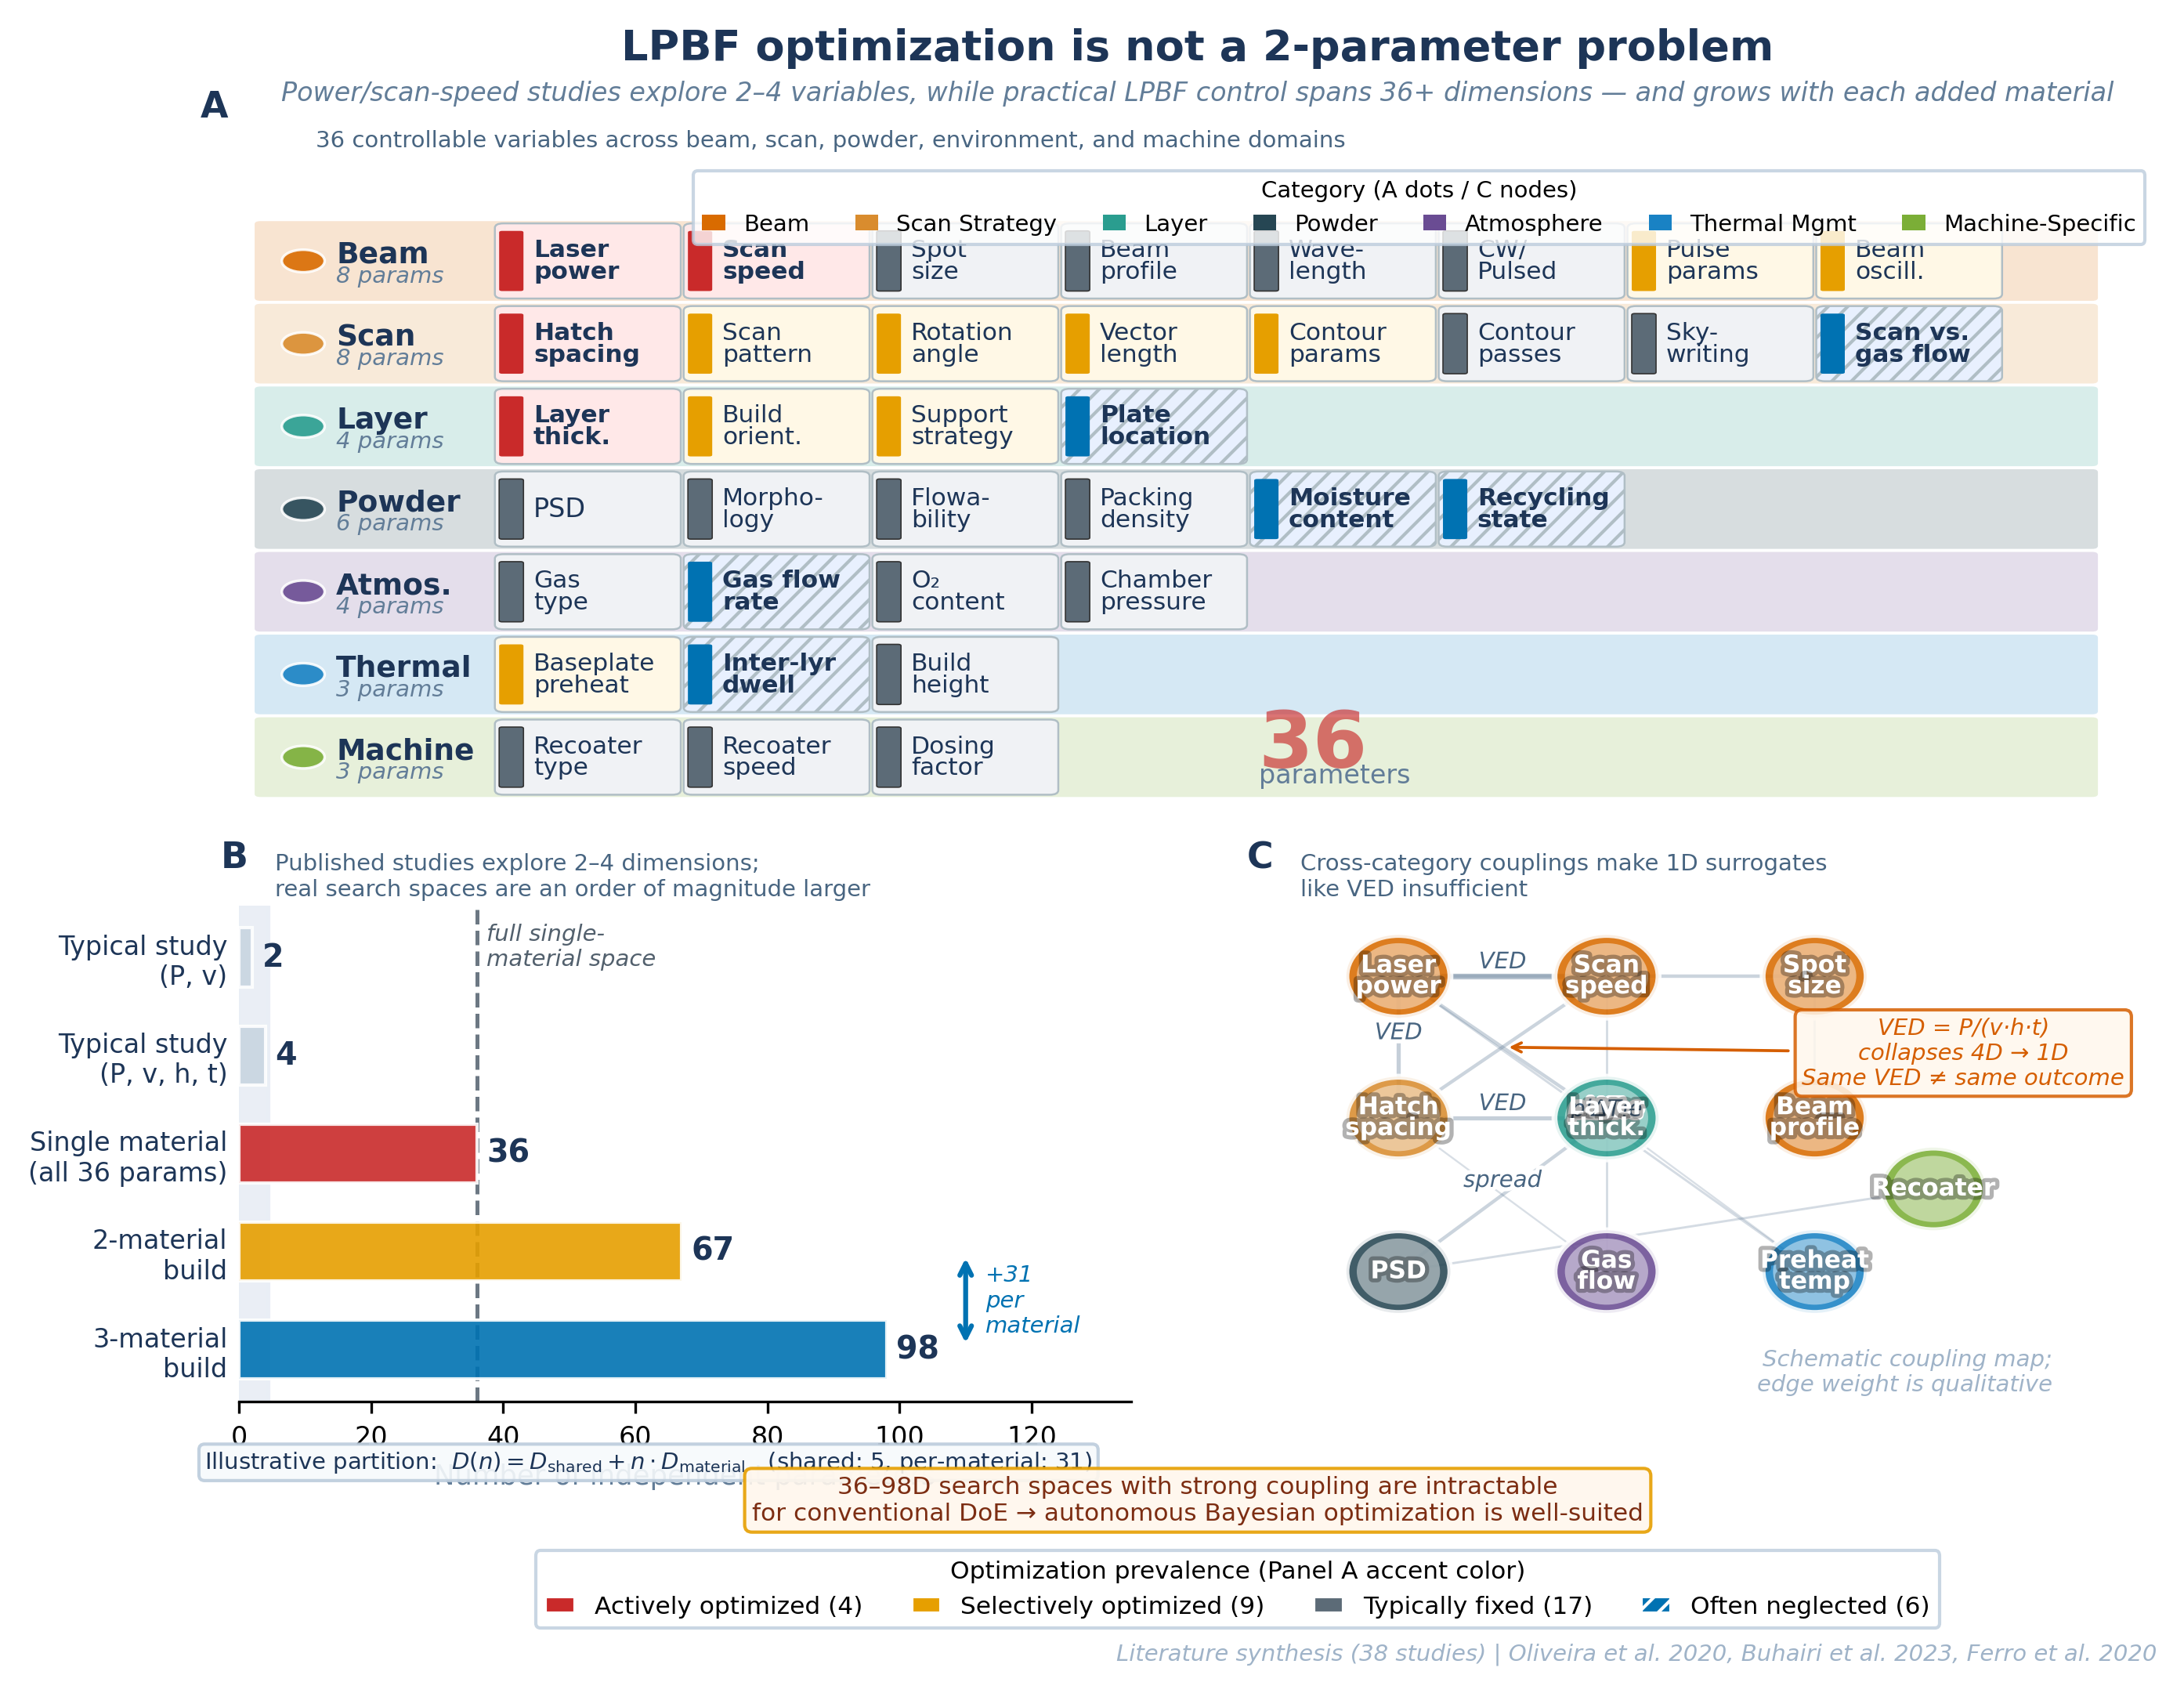
\includegraphics[width=0.85\textwidth]{../figures/lpbf_parameter_space.png}
  \caption{LPBF parameter space taxonomy. Tile grid showing the 36 key process parameters organized by category (laser, powder, geometry, atmosphere, post-processing), illustrating the high-dimensional optimization space addressed by FLAIME's BOFN framework.}
  \label{fig:lpbf-params}
\end{figure}

\begin{figure}[ht]
  \centering
  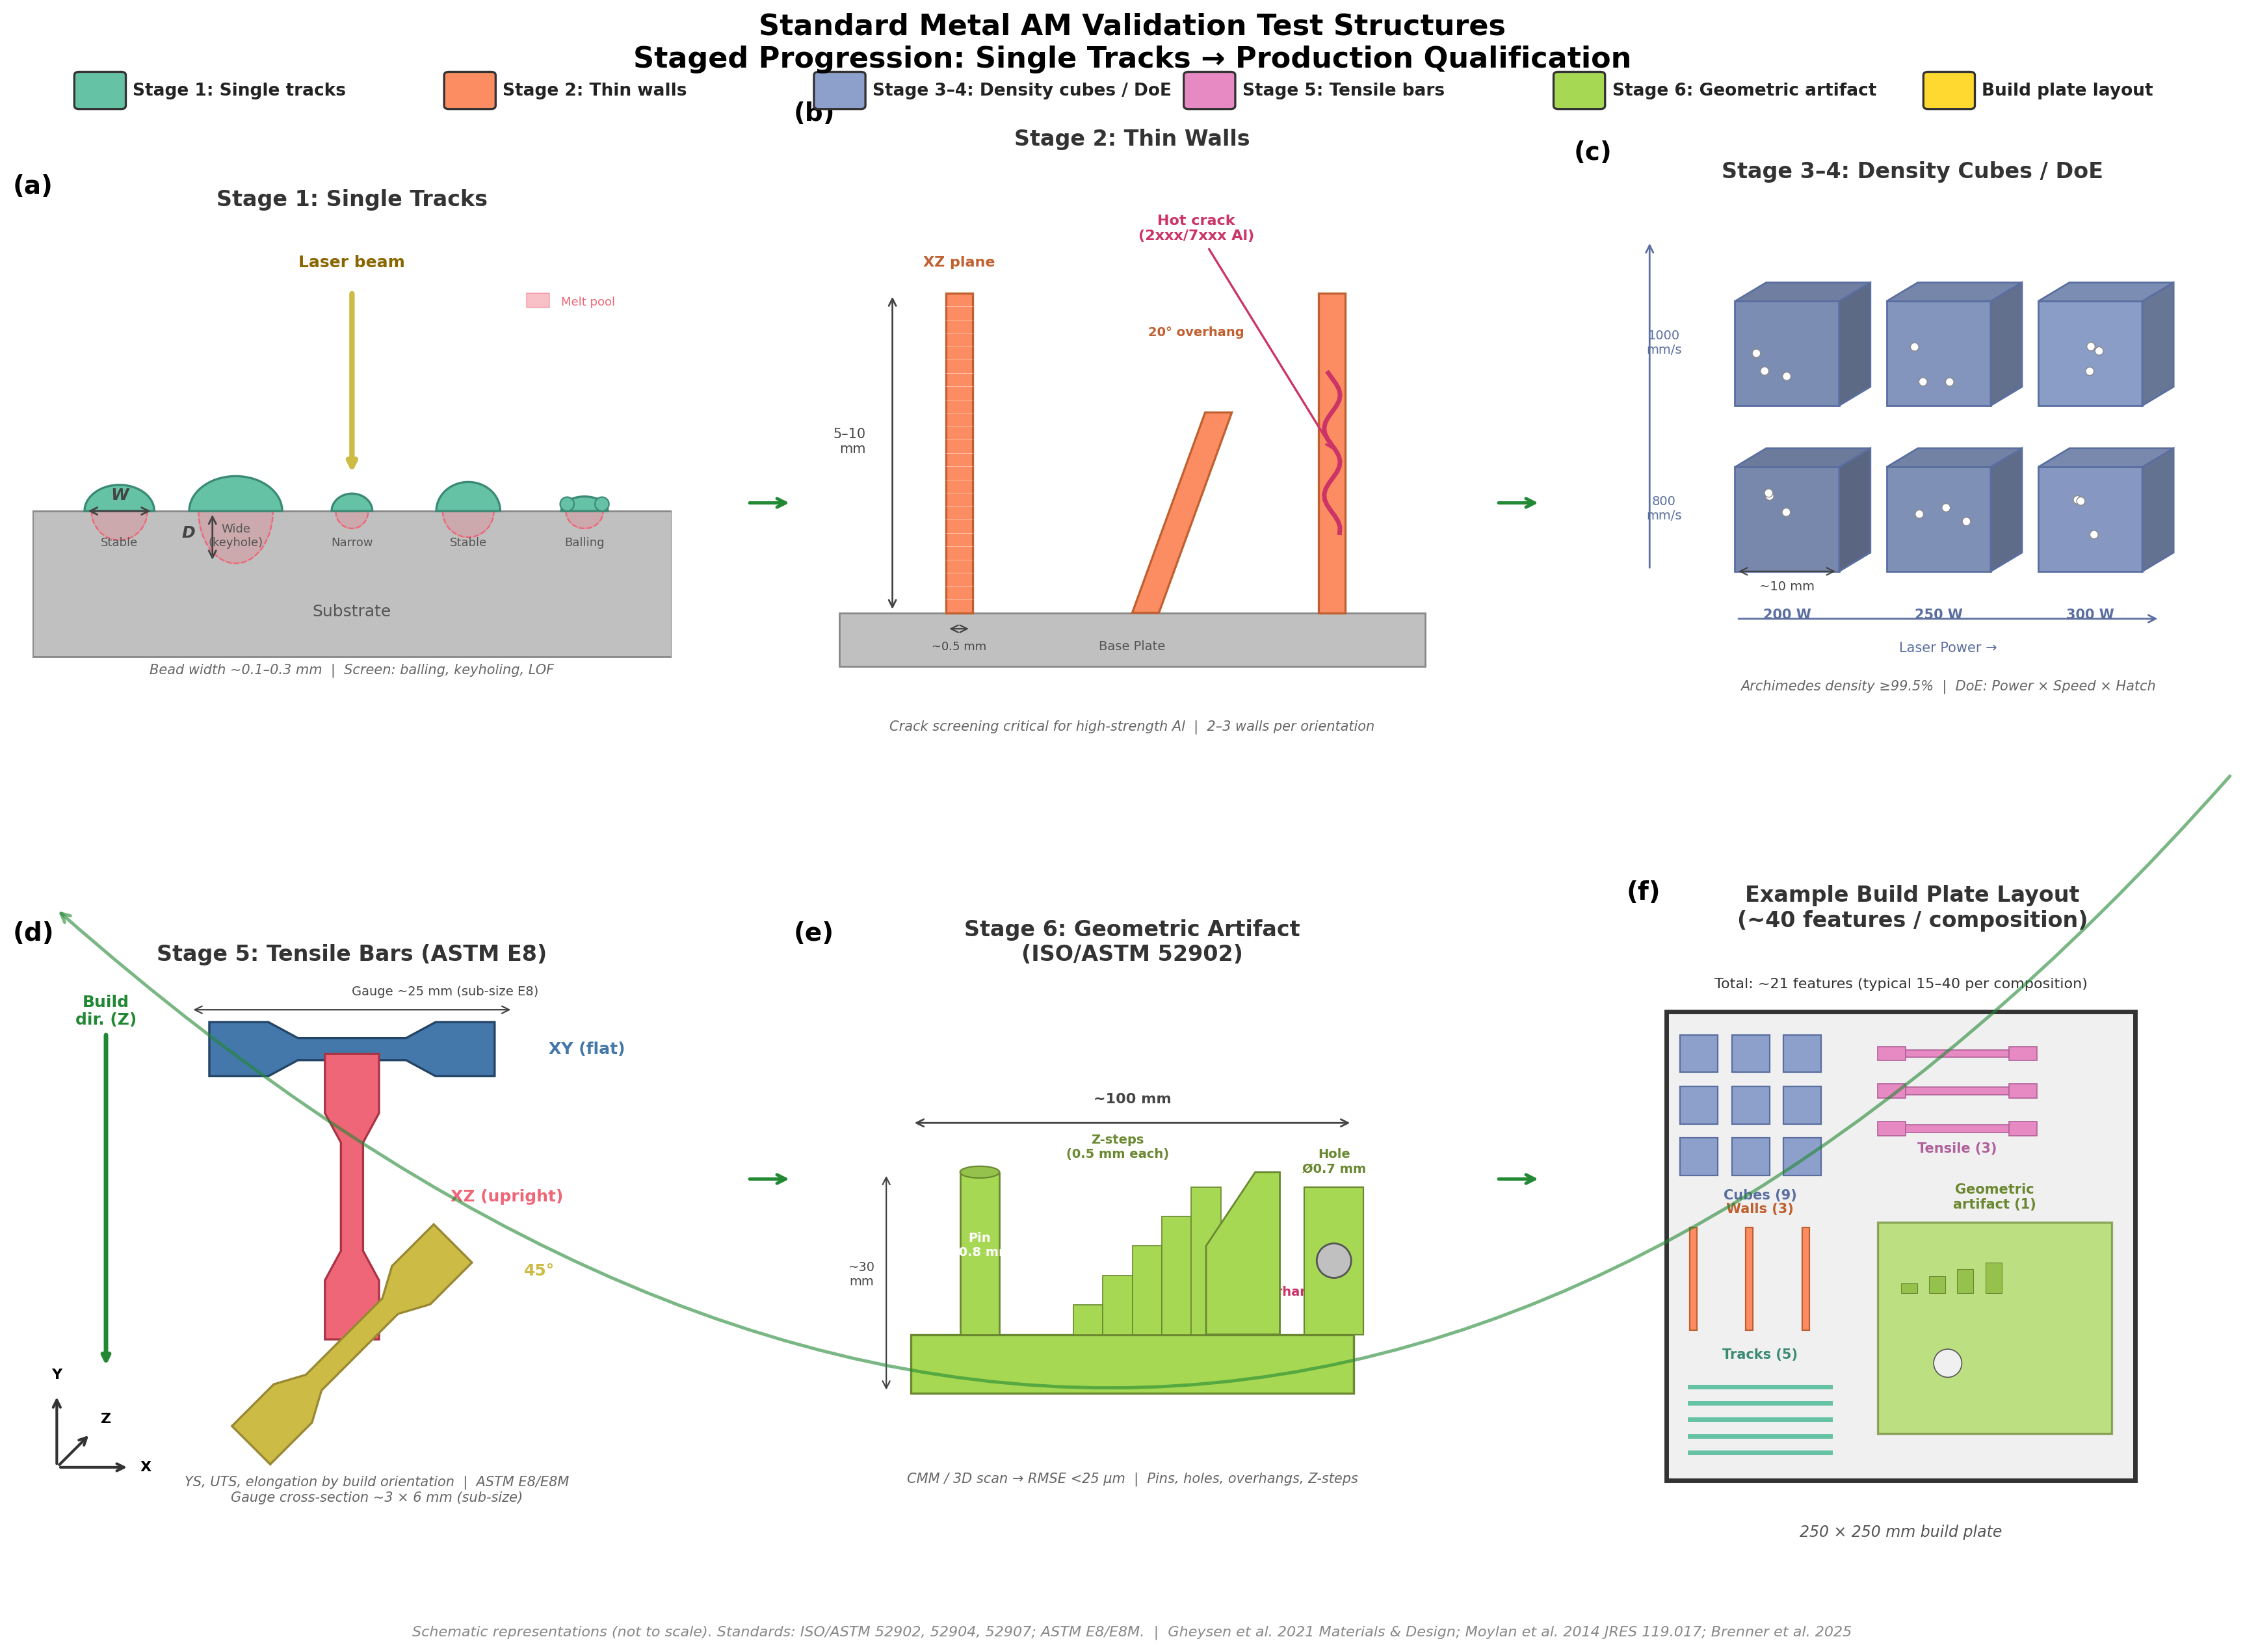
\includegraphics[width=0.85\textwidth]{../edison-trajectories/fig-am-test-structures-schematics.png}
  \caption{AM test structure progression. Build plate layout schematics showing the minimum viable specimen (MVS) hierarchy: single tracks for melt pool characterization, $5\times5\times5$\,mm density cubes for densification screening ($\geq$99\% relative density gate), and ASTM~E8 sub-size tensile bars for mechanical property evaluation.}
  \label{fig:am-test-structures}
\end{figure}

\begin{figure}[ht]
  \centering
  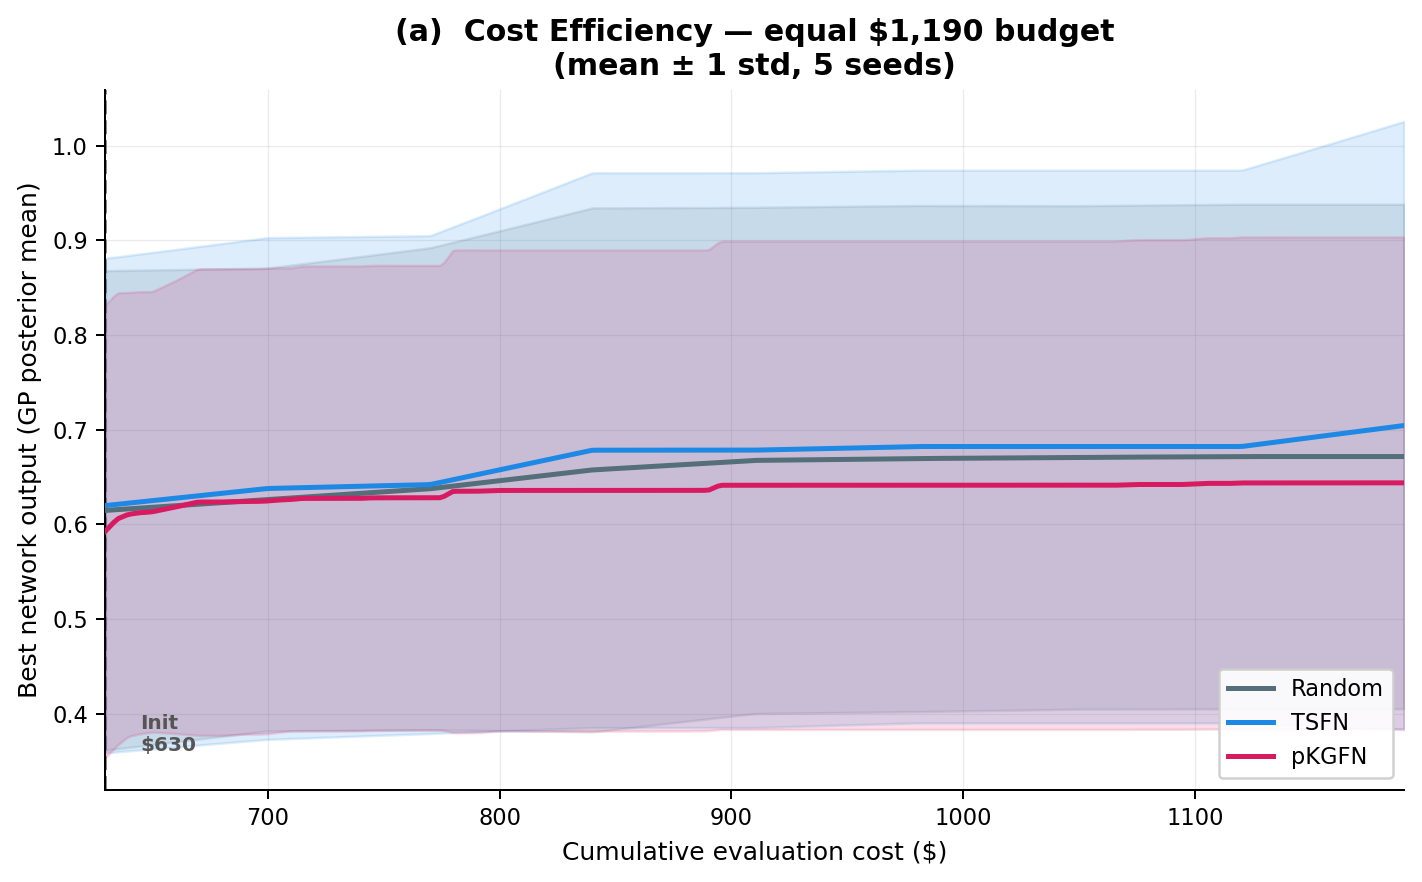
\includegraphics[width=0.85\textwidth]{../benchmarks/figures/pkgfn_cost_efficiency.png}
  \caption{Supplementary pKGFN benchmark result showing cost-aware evaluation performance versus standard acquisition functions.}
  \label{fig:pkgfn-supplementary}
\end{figure}

\begin{figure}[!htbp]
  \centering
  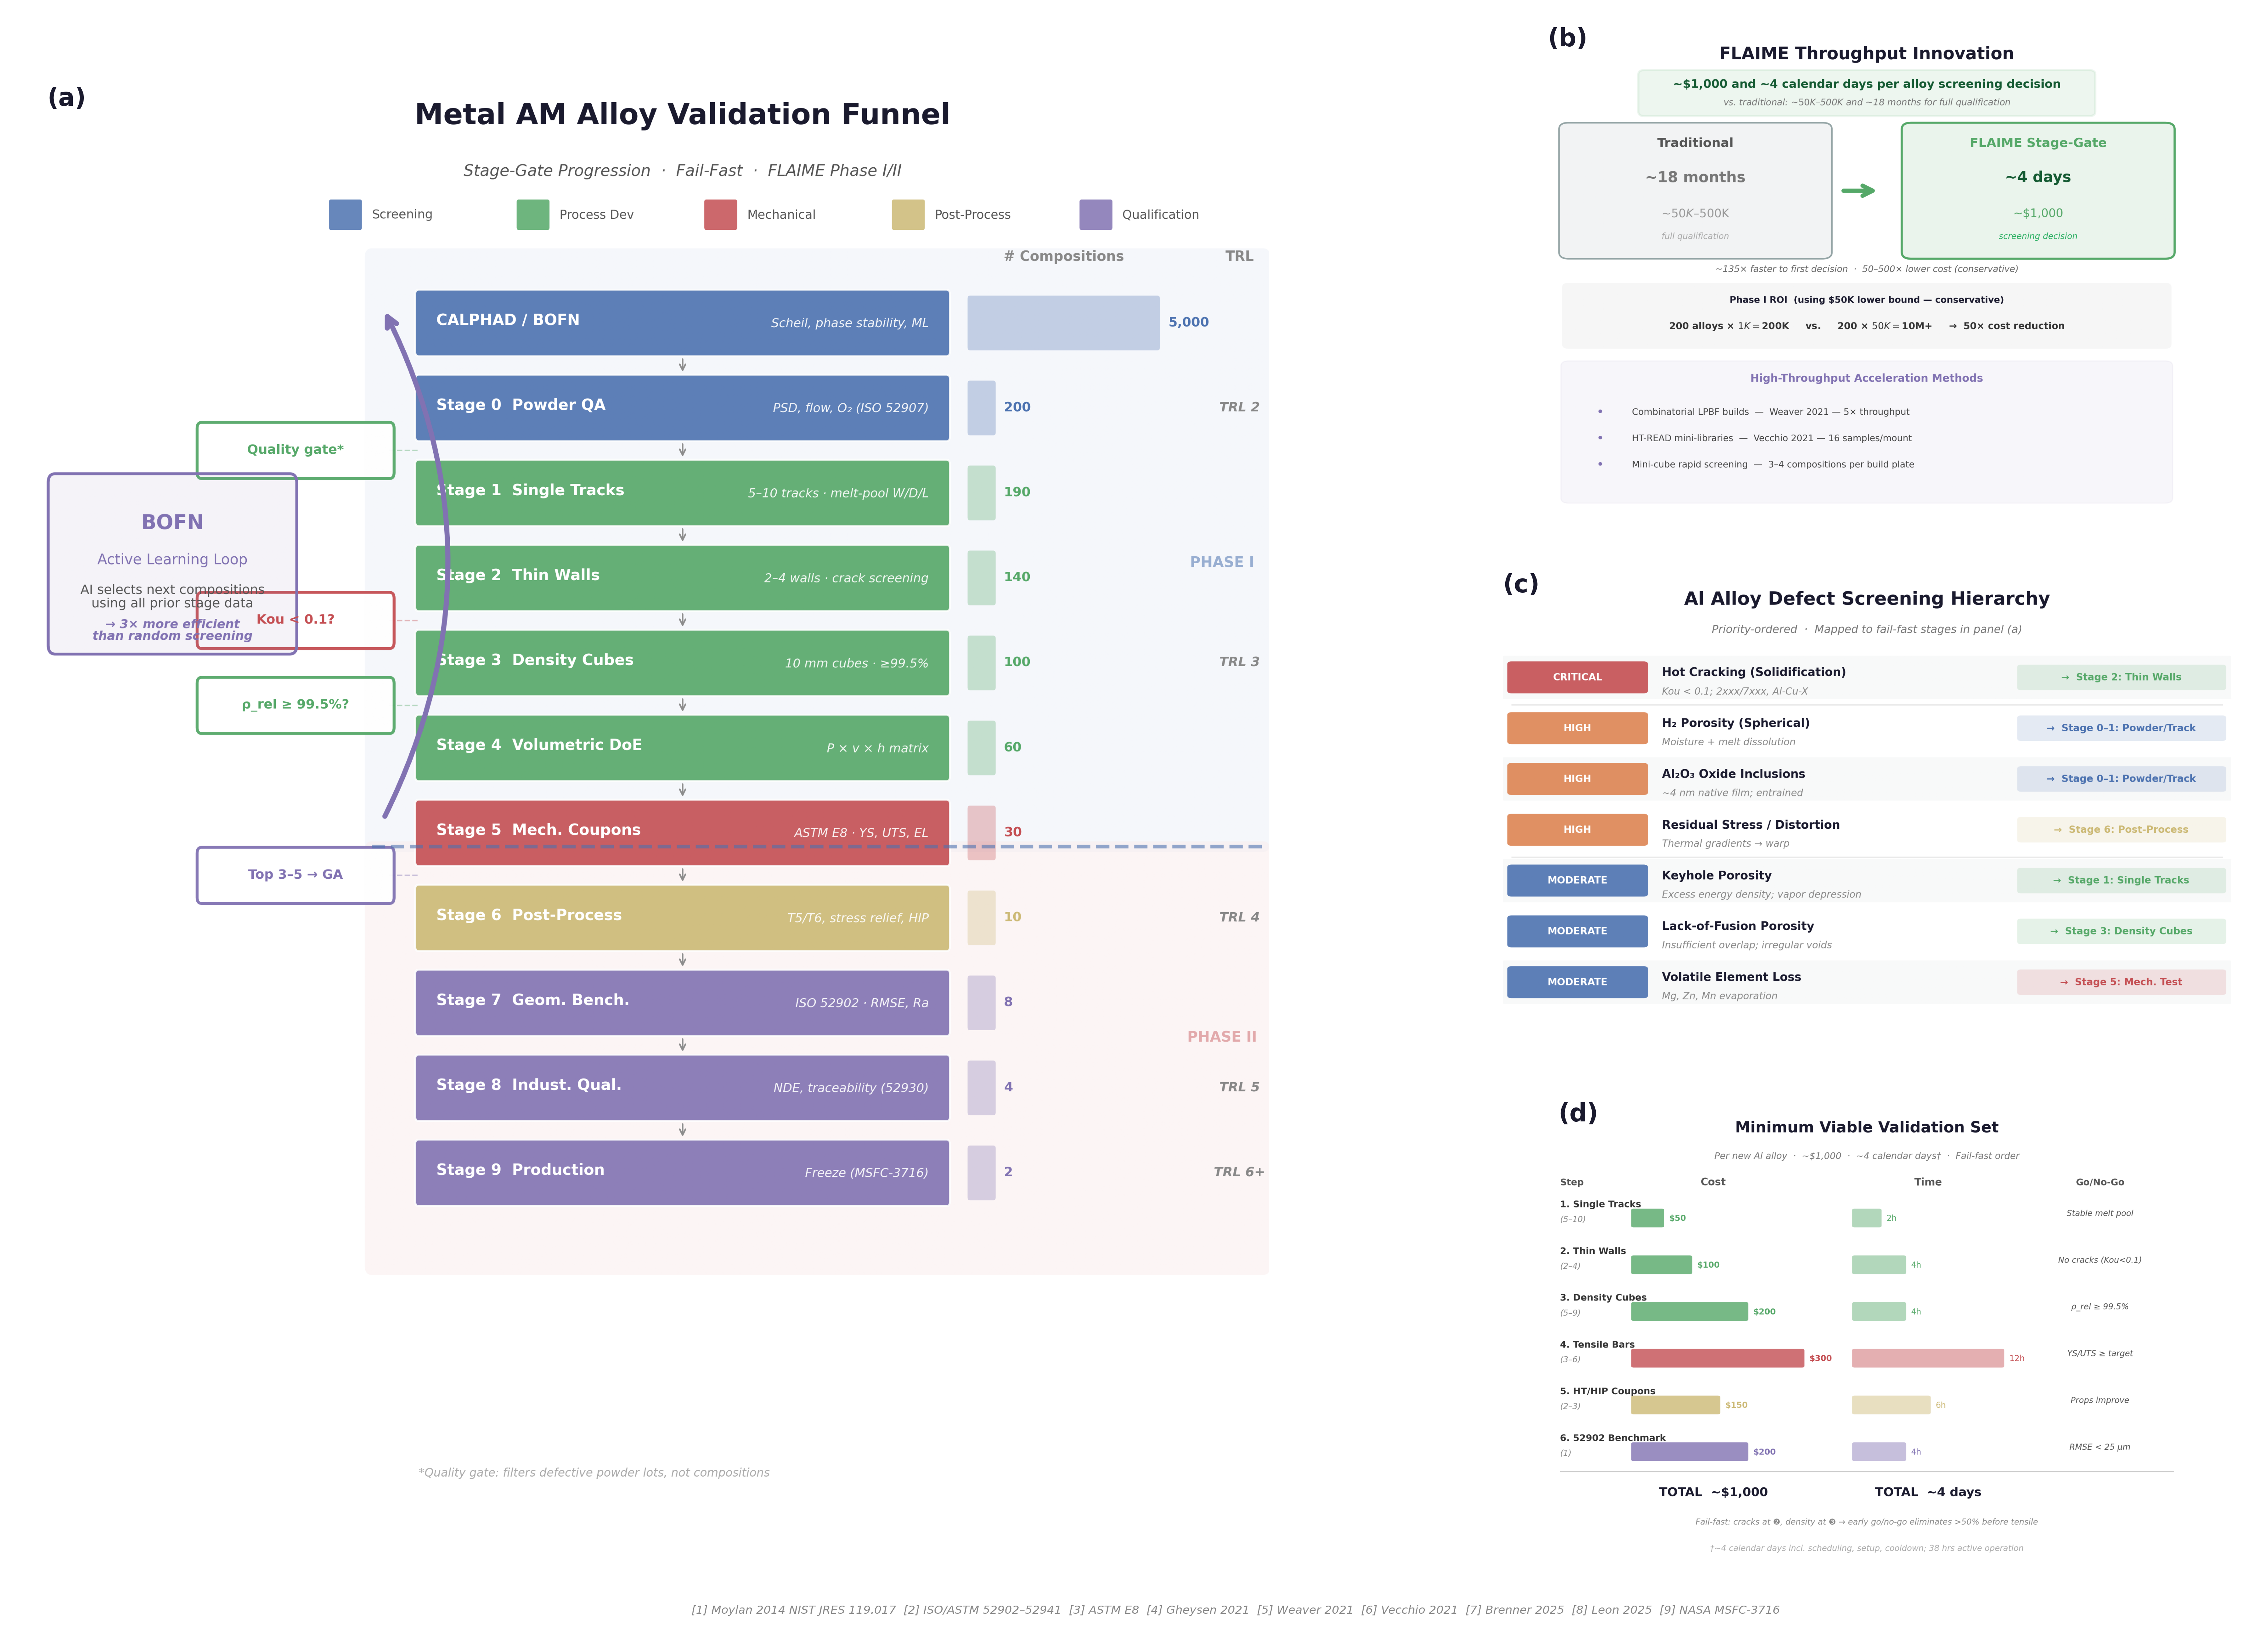
\includegraphics[width=0.85\textwidth]{../figures/composite_4panel.png}
  \caption{FLAIME experimental framework (overview figure relocated from Methods for narrative page-budget compliance): (a)~multi-fidelity stage-gate pipeline with fail-fast screening, (b)~throughput vs.\ traditional alloy development, (c)~Al alloy defect screening hierarchy, (d)~minimum viable validation set per alloy.}
  \label{fig:composite}
\end{figure}

\bigskip\noindent\rule{\textwidth}{0.4pt}

% ============================================================================
%  APPENDIX 3: EQUIPMENT
%  (0.5 page max; does NOT count against narrative limit)
% ============================================================================
\section*{Appendix 3: Equipment}
\label{app:equipment}

\required{FOA \S IV.C: ``List major items of equipment planned for use
in this project and, if appropriate, identify location and pertinent
capabilities.''  Maximum one page per institution.}

\smallskip\noindent
Major equipment is grouped by general workflow categories.

% ---------- POWDER PRODUCTION ----------
\medskip\noindent\textbf{\textsc{Powder Production}}

\noindent
\begin{minipage}[t]{0.62\textwidth}\raggedright
\textbf{AMAZEMET rePOWDER Ultrasonic Atomizer with Induction Crucible
Module} (BYU; delivery April~30, 2026).  Custom Al alloy powder production
from elemental powder mixtures packed into machined high-purity Al
crucibles; enables up to 3 compositions/day (M--F) and 1 on Saturday.\\[3pt]
\textbf{Aconity MIDI LPBF System} (UofU, Prof.\ Spear).
170\,mm \textsf{\O} build plate, open-parameter architecture,
200--1000\,W fiber laser; ideal for rapid alloy screening.  The
open-parameter framework maps directly to Thermo-Calc AM~Module
tunable parameters.
\end{minipage}\hfill
\begin{minipage}[t]{0.17\textwidth}
\centering
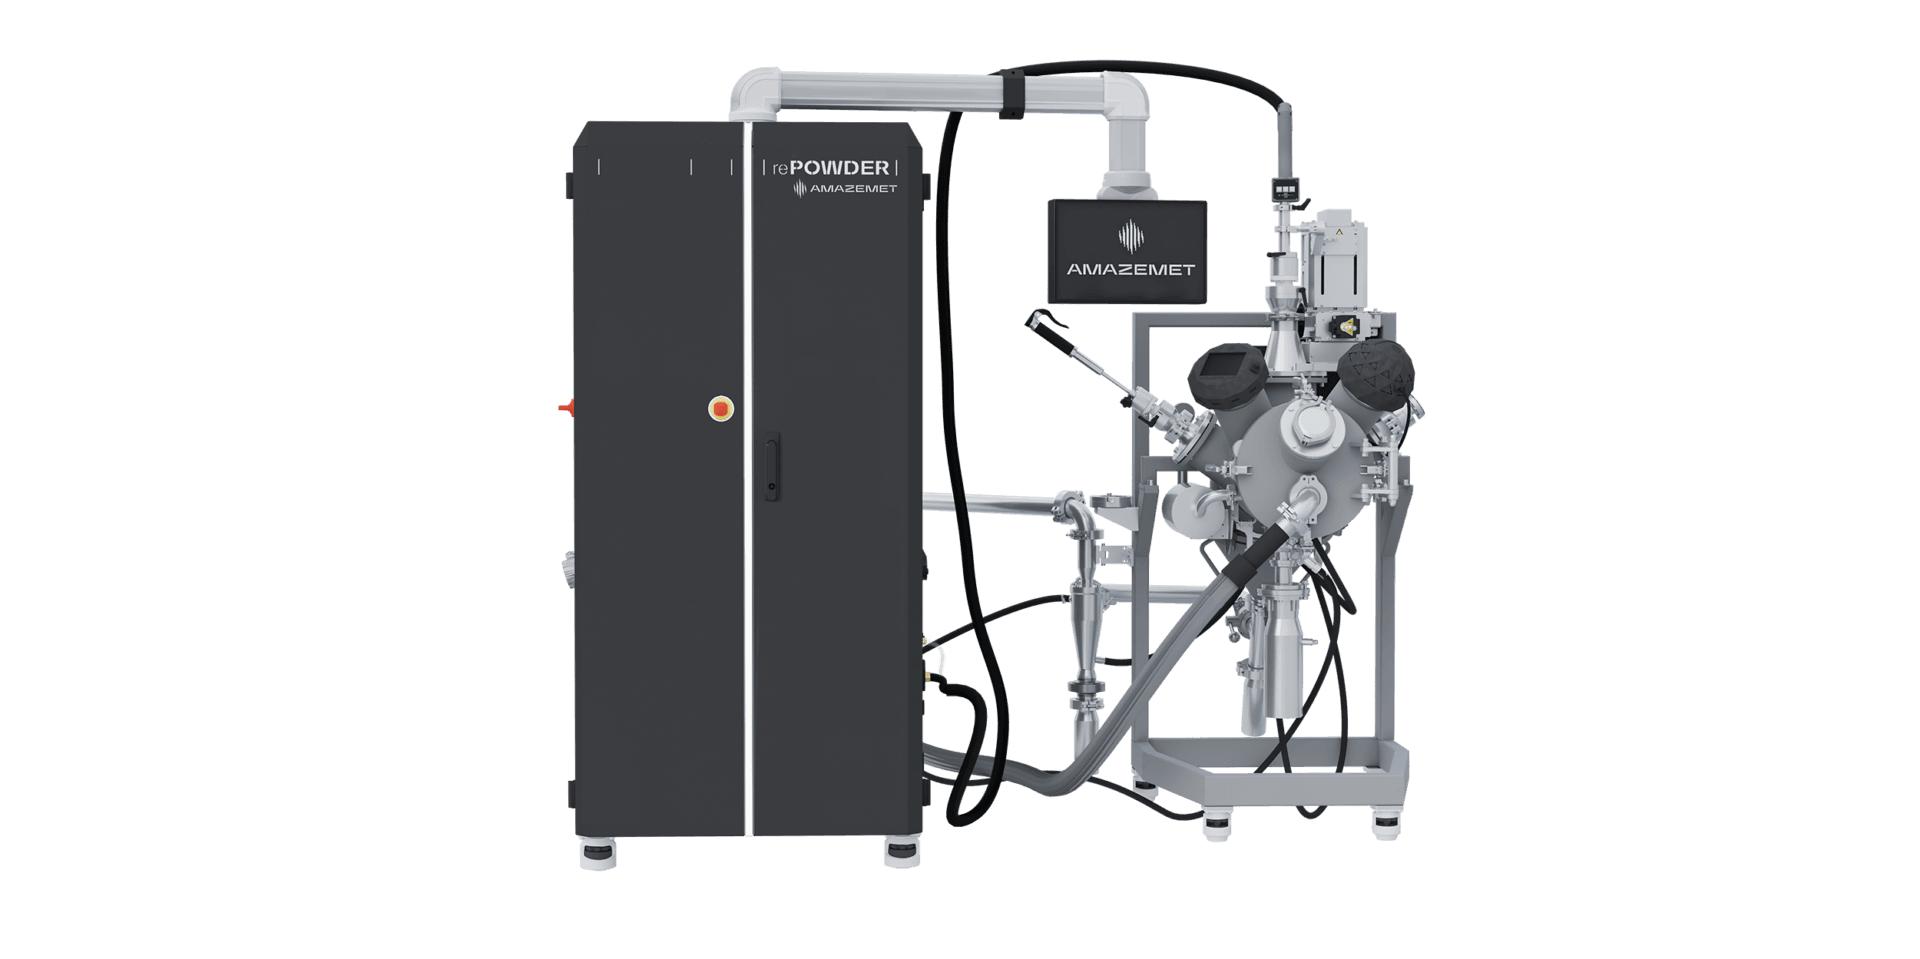
\includegraphics[width=\linewidth]{amazemet-repowder}\\[-2pt]
{\tiny AMAZEMET rePOWDER}
\end{minipage}\hfill
\begin{minipage}[t]{0.17\textwidth}
\centering
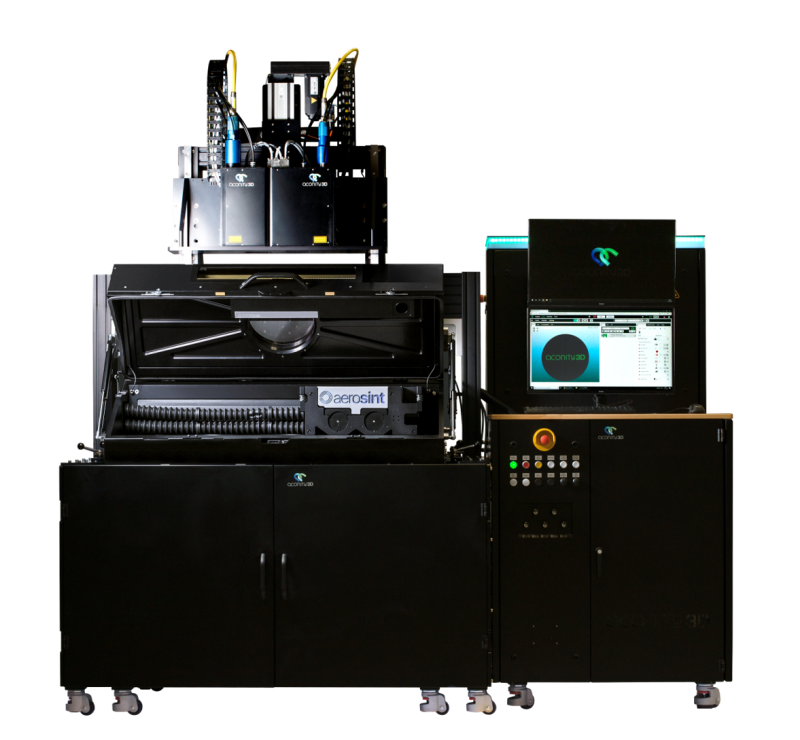
\includegraphics[width=\linewidth]{aconity-midi}\\[-2pt]
{\tiny Aconity MIDI}
\end{minipage}

% ---------- CHARACTERIZATION ----------
\medskip\noindent\textbf{\textsc{Characterization \& Microscopy}}

\noindent
\begin{minipage}[t]{0.62\textwidth}\raggedright
\textbf{BYU Microscopy Center SEM Suite:}\\
\begin{tabular}{@{}lcccc@{}}
\tiny & \tiny Tecnai & \tiny Verios & \tiny Helios & \tiny Apreo~C \\
\tiny & \tiny TF-20 TEM & \tiny SEM & \tiny 600 & \tiny SEM \\
\tiny ETD & & $\checkmark$ & $\checkmark$ & $\checkmark$ \\
\tiny BSE & & $\checkmark$ & & $\checkmark$ \\
\tiny EDS & $\checkmark$ & $\checkmark$ & $\checkmark$ & $\checkmark$ \\
\tiny EBSD & & & $\checkmark$ & $\checkmark$ \\
\tiny CL & & & & $\checkmark$ \\
\tiny FIB & & & $\checkmark$ & \\
\tiny STEM & $\checkmark$ & $\checkmark$ & & \\
\end{tabular}\\[3pt]
\textbf{Keyence VHX-7000 Optical Microscope} (BYU).
High-resolution digital microscope with automated tiling,
depth-of-field composition, and quantitative measurement;
metallography and defect screening.\\[3pt]
\textbf{BYU XRD Facility}
(\url{https://labs.chem.byu.edu/xrd-facility}).  Phase identification
and crystallographic analysis.\\[3pt]
\textbf{BYU Spectroscopic Facility:} XPS surface analysis
(\url{https://labs.chem.byu.edu/byu-spectroscopic-facility/surface-analysis});
\textbf{Agilent 8900 ICP-MS/MS}
(\url{https://labs.chem.byu.edu/byu-spectroscopic-facility/atomic-analysis})
for authoritative elemental composition verification.
\end{minipage}\hfill
\begin{minipage}[t]{0.35\textwidth}
\centering
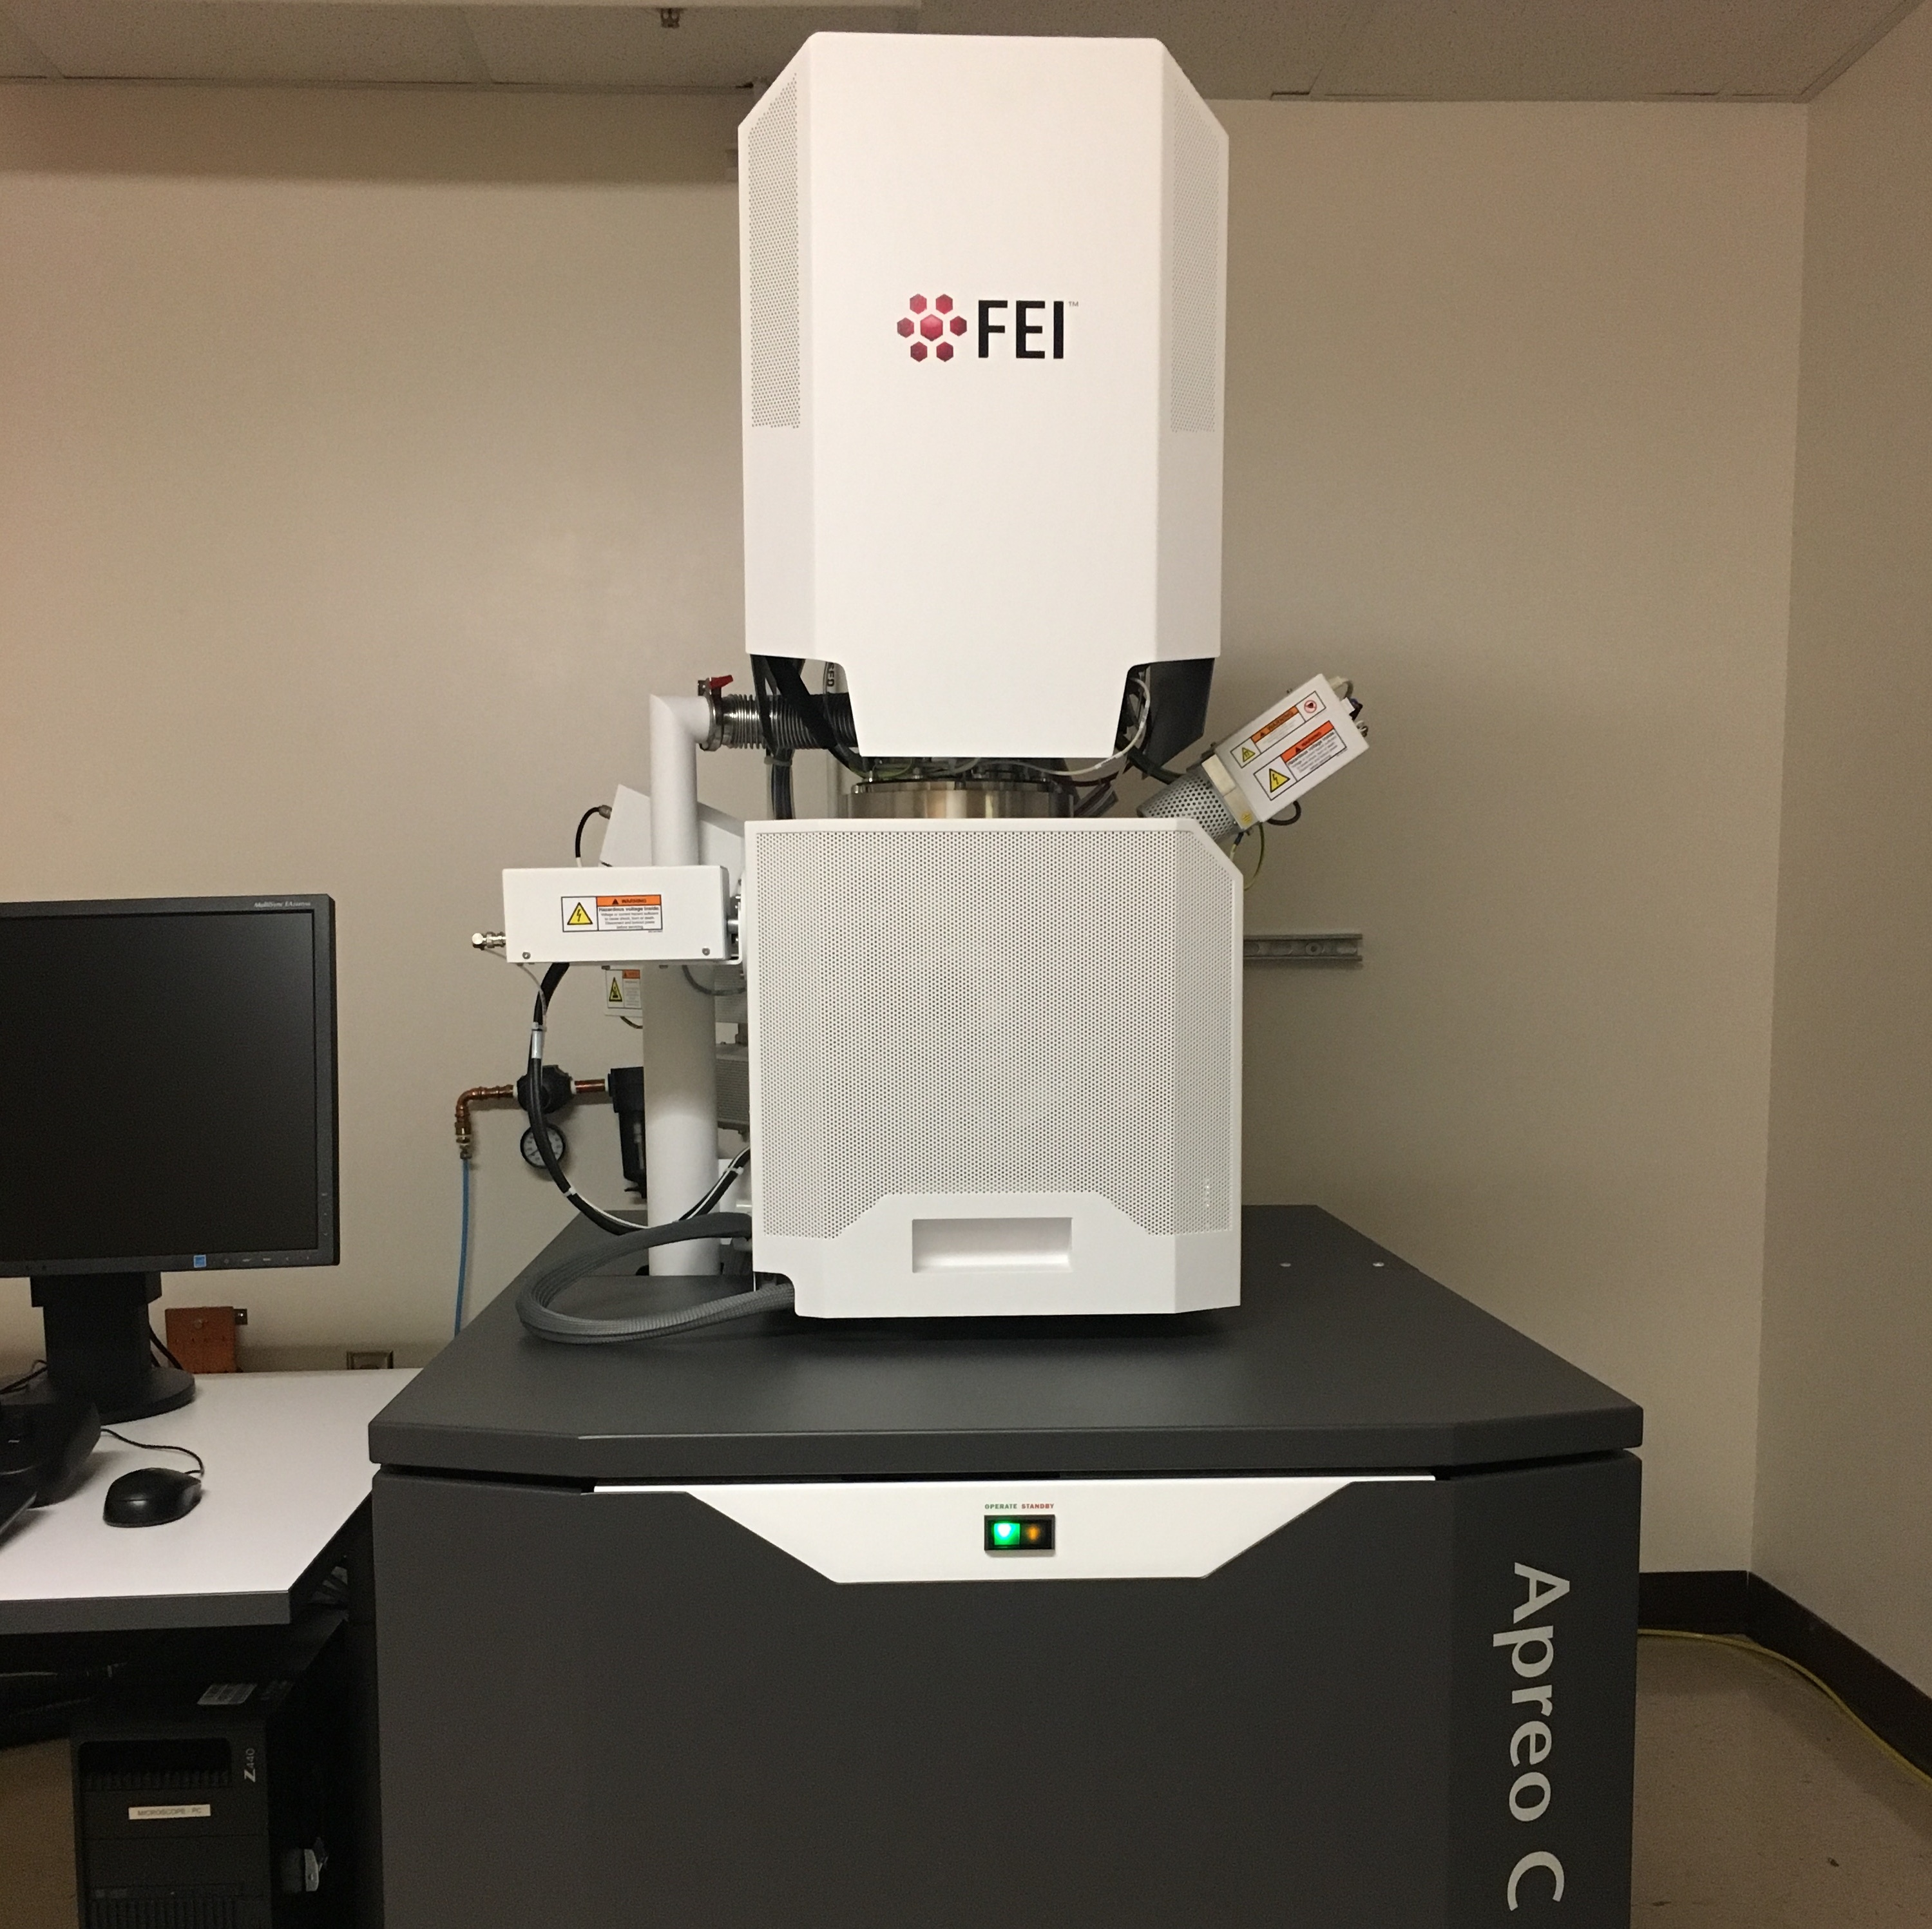
\includegraphics[width=0.48\linewidth]{apreo-sem}%
\hfill
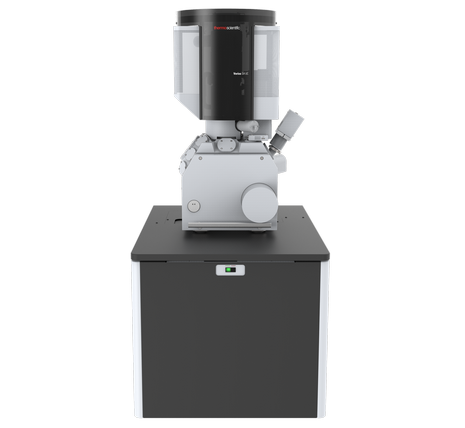
\includegraphics[width=0.48\linewidth]{verios-sem}\\[-2pt]
{\tiny Apreo~C SEM \hfill Verios SEM}\\[3pt]
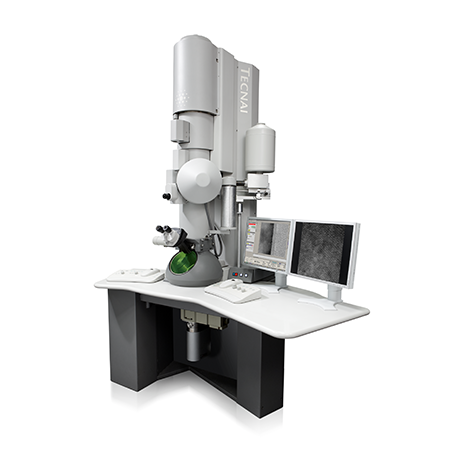
\includegraphics[width=0.48\linewidth]{tecnai-tf20-tem}%
\hfill
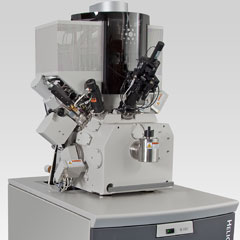
\includegraphics[width=0.48\linewidth]{helios-nanolab}\\[-2pt]
{\tiny Tecnai TF-20 TEM \hfill Helios 600}
\end{minipage}

% ---------- SAMPLE PREPARATION ----------
\medskip\noindent\textbf{\textsc{Sample Preparation}}

\noindent
\begin{minipage}[t]{0.62\textwidth}\raggedright
\textbf{Metallographic Polishing Lab} (BYU).
PX500 Automatic Polisher (1.5\textquotedbl{} sample pucks),
two PX300 Manual Polishers, non-crystallizing silica vibratory polishers,
fume hood for chemical etching, and electrochemical polisher (Lead PI
has extensive experience with all).  Metallographic polishing and
optical microscopy are both BOFN DAG nodes.\\[3pt]
\textbf{Rolling Mill} (BYU).  Resolution 0.00005\textquotedbl{},
width 6\textquotedbl{}.
\end{minipage}\hfill
\begin{minipage}[t]{0.35\textwidth}
\centering
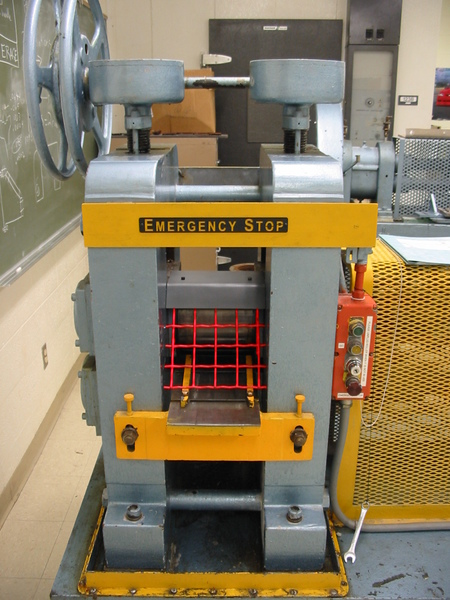
\includegraphics[width=0.9\linewidth]{rolling-mill}\\[-2pt]
{\tiny Rolling Mill}
\end{minipage}

% ---------- MECHANICAL TESTING ----------
\medskip\noindent\textbf{\textsc{Mechanical Testing}}

\noindent
\begin{minipage}[t]{0.62\textwidth}\raggedright
\textbf{100\,kip Landmark Tensile Tester} (BYU).
Tensile/compressive loads; capacity 110{,}000\,lb ($\pm$10\,lb);
stroke 6\textquotedbl{} ($\pm$0.001\textquotedbl{});
specimen width 0--0.83\textquotedbl{},
diameter 0.25--2.02\textquotedbl{}.\\[3pt]
\textbf{20\,kip 809 A/T Tensile Tester} (BYU).
Tensile/compressive/torsional loads; axial capacity 20{,}000\,lb
($\pm$2\,lb); torsional capacity 10{,}000\,in$\cdot$lb.\\[3pt]
\textbf{Impact Tester: Instron Model SI-1D3} (BYU).
Striker weight 66.6\,lb; drop height 4.51\,ft; impact velocity
17\,ft/s; range 0--300\,ft-lbs.  Equipped for Charpy and Izod
impact tests.\\[3pt]
\textbf{Micro Hardness Indenter} (BYU).  Hardness and modulus mapping.\\[3pt]
\textbf{Zeiss Xradia Versa 620 Nano-CT} (UofU EMSAL).
Non-destructive 3D defect analysis; in-situ tensile stage
(5\,kN), heating/cooling capability, lab-DCT.
\end{minipage}\hfill
\begin{minipage}[t]{0.17\textwidth}
\centering
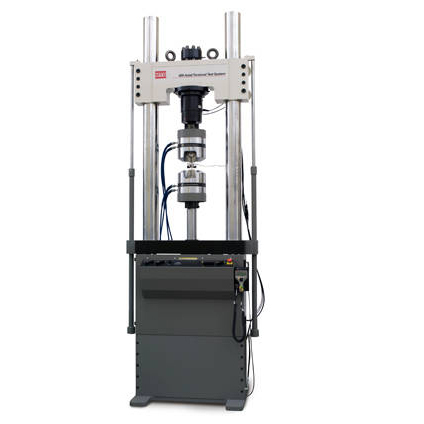
\includegraphics[width=\linewidth]{tensile-100kip}\\[-2pt]
{\tiny 100\,kip Landmark}
\end{minipage}\hfill
\begin{minipage}[t]{0.17\textwidth}
\centering
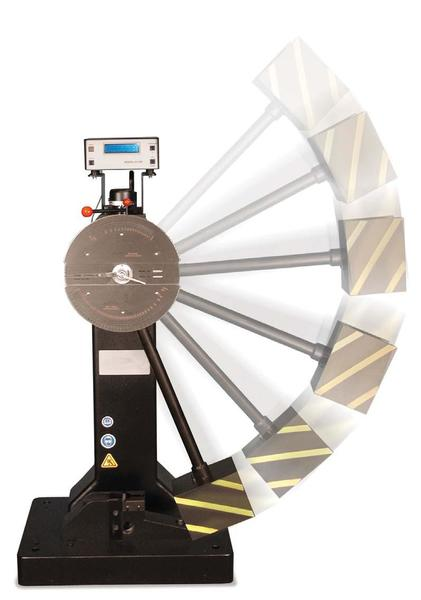
\includegraphics[width=\linewidth]{impact-tester}\\[-2pt]
{\tiny Instron SI-1D3}
\end{minipage}

% ---------- HEAT TREATMENT ----------
\medskip\noindent\textbf{\textsc{Heat Treatment}}

\noindent
\begin{minipage}[t]{0.62\textwidth}\raggedright
\textbf{Recco Furnace} (BYU).
Capacity 12\textquotedbl{}W $\times$ 7\textquotedbl{}H $\times$
19\textquotedbl{}D; max temperature 2250\textdegree{}F;
Ar/N$_2$ atmosphere capability.\\[3pt]
\textbf{Lucifer Furnace} (BYU, CB~121).
Capacity 10\textquotedbl{}W $\times$ 8\textquotedbl{}H $\times$
18\textquotedbl{}D; max temperature 2350\textdegree{}F.\\[3pt]
\textbf{MTI Vacuum Furnace} (BYU).
Capacity 40\,mm diameter $\times$ 200\,mm length; max temperature
1100\textdegree{}C (1000\textdegree{}C continuous); vacuum level
$5.0\times10^{-3}$\,mbar.\\[3pt]
\textbf{CM Hydrogen Furnace} (BYU).
Capacity 3\textquotedbl{} diameter; max temperature 1600\textdegree{}C;
hydrogen, nitrogen, ethylene, and air atmospheres.\\[3pt]
\textbf{Custom Ultra-High-Purity Induction Tube Furnace} (built by Lead PI).
Semi-automated with PID temperature ramping (including rapid ramp/cool);
high-vacuum (turbomolecular pump) or backfilled inert gas;
non-contact 2-color pyrometer through replaceable quartz windows;
custom crucibles/susceptors with sapphire windows.
Max temperature 2500\textdegree{}C.
\end{minipage}\hfill
\begin{minipage}[t]{0.35\textwidth}
\centering
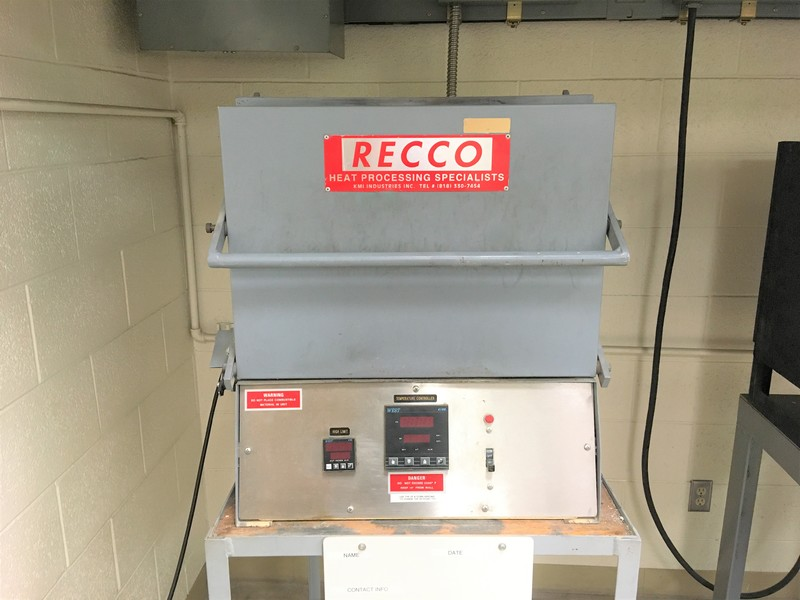
\includegraphics[width=0.45\linewidth]{recco-furnace}%
\hfill
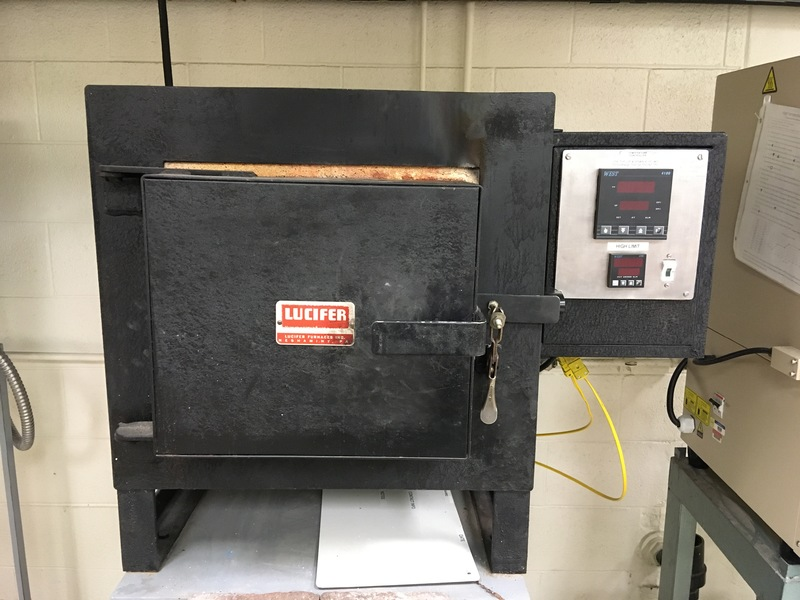
\includegraphics[width=0.45\linewidth]{lucifer-furnace}\\[-2pt]
{\tiny Recco \hfill Lucifer}\\[3pt]
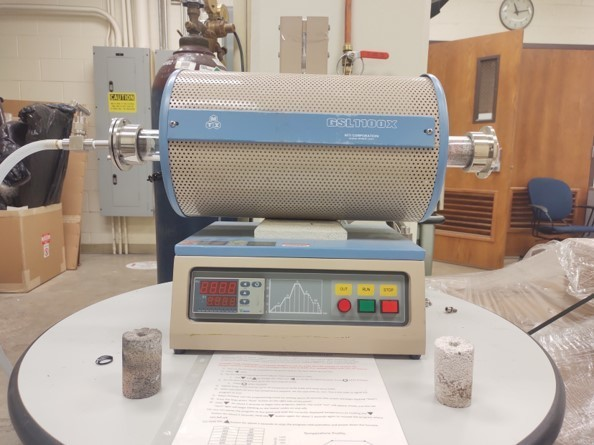
\includegraphics[width=0.45\linewidth]{mti-vacuum-furnace}%
\hfill
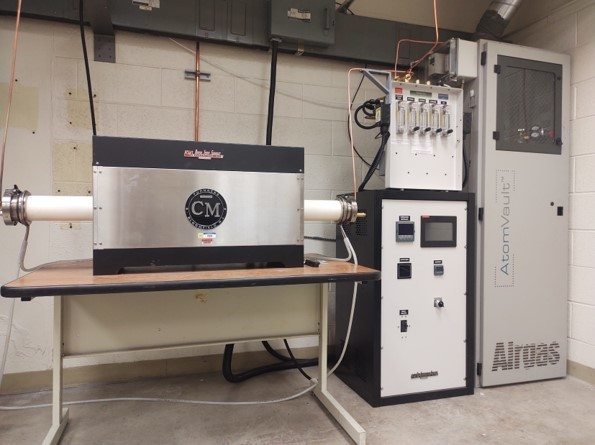
\includegraphics[width=0.45\linewidth]{cm-hydrogen-furnace}\\[-2pt]
{\tiny MTI Vacuum \hfill CM Hydrogen}
\end{minipage}

% ---------- COMPUTING ----------
\medskip\noindent\textbf{\textsc{Computing}}

\noindent
\begin{minipage}[t]{0.62\textwidth}\raggedright
\textbf{BYU HPC Cluster} (28K+ cores, 367~GPUs incl.\ H200/H100/A100,
SLURM).  No direct cost via fairshare scheduling.
Supports parallelized TC-Python CALPHAD sweeps and
BoTorch/GPyTorch surrogate training.
\end{minipage}\hfill
\begin{minipage}[t]{0.35\textwidth}
\centering
% HPC cluster image not available; text description sufficient.
\end{minipage}

% ============================================================================
%  APPENDIX 4: DATA MANAGEMENT AND SHARING PLAN (DMSP)
%  (NOT required at submission; required during award negotiation)
% ============================================================================
\newpage
\section*{Appendix 4: Data Management and Sharing Plan}
\label{app:dmsp}

\note{FOA \S IV.C: ``A Data Management and Sharing Plan (DMSP) is NOT
required as an appendix to the project narrative but it will be required
during award negotiation.''  This section is included for planning
purposes only.  You may request DMSP implementation costs in the budget.}

\guidance{When preparing the DMSP for award negotiation, it must address
(per FOA \S IV.C): (1) How FAIR principles will apply to datasets,
software, and models; (2) what will be released under open-source
licenses (specify SPDX identifiers); (3) how best practices in scientific
software development will be applied (see bssw.io).}

\textbf{1.\ Types of Data.} \flaime{} will generate: (i)~alloy composition
data (wt\%/at\% of Al, Mn, Cr, Zr via ICP-OES); (ii)~CALPHAD simulation
outputs (phase diagrams, Scheil--Gulliver curves, solidification parameters
from Thermo-Calc TCAl10/AM~Module); (iii)~powder characterization records
(PSD, SEM/EDS, flowability); (iv)~LPBF processing parameters (power, speed,
hatch spacing, layer thickness) and build metadata; (v)~mechanical properties
(YS, UTS, elongation per ASTM~E8/E8M) and microstructural images (SEM,
EBSD); and (vi)~BOFN/pKGFN model parameters, acquisition function logs, and
digital thread provenance records.

\textbf{2.\ Data Formats.} Tabular data will be stored in CSV/JSON with
schema.org metadata. Large simulation arrays will use HDF5. Microscopy
images will be archived as lossless TIFF. ML models will be serialized in
ONNX for interoperability.

\textbf{3.\ Sharing and Preservation.} All experimental datasets will be
deposited on Zenodo and/or Figshare with DOIs within 12~months of
collection. The \flaime{} digital thread will be hosted on the American
Science Cloud (AmSC) per Genesis Mission requirements. Software
(BOFN/pKGFN engine, Honegumi tutorials) will be released on GitHub under
MIT/Apache-2.0 licenses, following bssw.io best practices.

\textbf{4.\ Access and Reuse.} Data and models will adhere to FAIR
principles. Datasets will carry schema.org metadata for machine
discoverability. Data licensed CC-BY-4.0; code licensed MIT. Supply-risk
metadata (Helbig SRI scores) will be linked to every composition record.

\textbf{5.\ Oversight.} The PI is responsible for DMSP compliance. Quarterly
data audits will be conducted throughout Phase~I. Budget provisions for data
curation, DOI registration, and AmSC hosting are included under Other
Direct Costs.

% ============================================================================
%  APPENDIX 5: SYNERGISTIC ACTIVITIES (Optional)
%  (1 page per senior/key person; does NOT count against narrative limit)
% ============================================================================
\newpage
\section*{Appendix 5: Synergistic Activities}
\label{app:synergistic}

\note{FOA \S IV.C: Optional. ``Each senior/key person has the option to
provide a one-page list of no more than five distinct examples of
synergistic activities that demonstrate the individual's professional
and scholarly activities that focus on the integration, transfer, and
creation of knowledge as related to the application.''  Total pages
$\leq$ number of senior/key personnel.}

\begin{enumerate}

\item \textbf{Self-Driving Laboratory Leadership \& Community Building.}
Serving as Guest Editor for \textit{npj Computational Materials} for the
``Self-Driving Labs for Chemistry and Materials Science'' collection
(2024--present) and lead author of the structural materials section of a
comprehensive \textit{Chemical Reviews} review on self-driving laboratories
(Tom et al., 2024). Lead author of a review on low-cost self-driving
laboratories introducing the ``Frugal Twin'' concept (Lo et al., 2024,
\textit{Digital Discovery}). Solo-organized the Acceleration Consortium
Bayesian Optimization Hackathon (120 participants, 62 organizations,
14 countries).

\item \textbf{Open-Source Software \& Community Infrastructure.}
Contributed over 17,000 open-source code artifacts (15K commits, 1.5K
issues, 913 pull requests) spanning materials informatics, Bayesian
optimization, and laboratory automation. Developer of Honegumi, an
interactive Bayesian optimization script generator for experimental
scientists (JOSS, 2025), and xtal2png, a crystal-structure-to-image encoding
tool for generative modeling (JOSS, 2022). Served as Technical Consultant to
Meta for the v1.0 release of the Ax/BoTorch platform (Nov 2024--Jan 2025).
Over 350 self-driving lab demonstration kits deployed worldwide.

\item \textbf{Training \& Workforce Development.}
Delivered approximately 5,000 person-hours of self-driving laboratory
training to roughly 700 individuals across 62 organizations through
workshops, microcredential courses, and hackathons. Built the Acceleration
Consortium Development Lab from the ground up (\$600K in equipment, 500 line
items, 24 months). Developed over 200 hours of course content in robotics,
data science, and AI-driven experimental design.

\item \textbf{Standardization \& Open Science.}
Co-organizer of the annual NSF Pathways to Open-Source Ecosystems (POSE)
workshop (2024, 2025, 2026). Contributing to
Acceleration Consortium community standards for
self-driving laboratory interoperability and advancing FAIR data practices
through schema.org metadata templates for SDL datasets. Presenter at the
German-Canadian Materials Acceleration Centre (GCMAC) Summer School (2024,
2025) and Review Panelist for the NSF TIP Directorate (2026).

\item \textbf{Open Data Impact \& Domain Expertise.}
Creator of the MPTS-52 time-based dataset split, widely adopted in the
crystal structure generative AI community, and developer of the
Matbench-genmetrics framework for standardized evaluation of generative
models (JOSS, 2024). Completed a \$34K industry research contract with
Fehrmann Materials GmbH applying machine learning to joint strength and
ductility prediction in aluminum alloys. Maintains curated open datasets on
Zenodo and Figshare with documented community reuse.

\end{enumerate}

% ============================================================================
%  APPENDIX 6: TRANSPARENCY OF FOREIGN CONNECTIONS
%  (Required; does NOT count against narrative limit)
% ============================================================================
\newpage
\section*{Appendix 6: Transparency of Foreign Connections}
\label{app:foreign}

\required{FOA \S IV.C: Required for all applicants and subrecipients.
IHEs and non-profits: respond only to items marked with (*) in the
template.  DOE/NNSA labs and domestic government entities are exempt.
Use the template at
\url{https://www.energy.gov/ia/transparency-foreign-connections}
or provide equivalent information with signature, date, and certification
statement.  Include a separate disclosure for the applicant and each
proposed subrecipient.}

\instruct{If any partner is non-US (e.g., AMAZEMET, Poland), provide
complete foreign connections disclosure.  Route through BYU sponsored
programs office.}

[Foreign connections disclosure to be completed via BYU sponsored programs
office using the DOE template. Separate disclosures required for BYU (lead)
Valimet (funded partner), AMAZEMET (funded partner), and Thermo-Calc AB (Sweden,
funded partner). All partners submit independent, coordinated applications;
foreign connections disclosure will be completed per the institutional
template requirements for each applicant.]

% ============================================================================
%  APPENDIX 7: OTHER ATTACHMENTS
%  (Letters of Commitment, etc.; does NOT count against narrative limit)
% ============================================================================
\section*{Appendix 7: Other Attachments}
\label{app:other}

\required{FOA \S IV.C: ``Include the required Letters of Commitment and
any optional letters of collaboration or access.  You may also include
any needed elaboration to your responses to questions 1--6 on the `Other
Project Information' document or information not easily accessible to a
reviewer.  However, do not use this appendix to circumvent the page
limitations of the application.''}

% ---------------------------------------------------------------------------
%  QUICK-REFERENCE GUIDE FOR COLLABORATORS
% ---------------------------------------------------------------------------
\medskip
\noindent\fbox{\parbox{\dimexpr\textwidth-2\fboxsep-2\fboxrule}{%
\small\textbf{Quick-Reference: Letter Types Required by this FOA
(DE-FOA-0003612)}\\[3pt]
The RFA specifies \textbf{two} types of letters. \emph{Letters of
recommendation / endorsement are \underline{not} allowed.}\\[4pt]
%
\begin{tabular}{@{}p{0.28\textwidth}p{0.68\textwidth}@{}}
\toprule
\textbf{Letter of Commitment} &
  Required from every institution \textbf{participating as a team member}
  (including the lead).
  Must be current, signed, and dated by a \textbf{person authorized to
  commit the institution to a legally binding agreement}.
  Maximum \textbf{one page}.
  Describes the nature of the institution's involvement. \\[3pt]
\textbf{Letter of Collaboration or Access} &
  Optional; from collaborators or institutions providing access to data,
  models, software, equipment, and/or facilities.
  Must follow a \textbf{strict 2-sentence format} (see template below).
  Must \underline{not} read as a recommendation or endorsement.
  No page limit stated, but brevity is expected. \\
\bottomrule
\end{tabular}\\[4pt]
\textit{All letters go in Appendix~7 (Other Attachments).
All letters may be addressed ``To Whom It May Concern.''}%
}}

% ---------------------------------------------------------------------------
%  WHO NEEDS WHAT
% ---------------------------------------------------------------------------
\medskip
\noindent\textbf{Letters needed for this proposal:}

\begin{enumerate}[leftmargin=*,nosep]\small
  \item \textbf{BYU} (lead institution) --- Letter of Commitment (signed by
        authorized university official, e.g.\ SPO or Dean)
  \item \textbf{Valimet, Inc.} (funded partner) --- Letter of Commitment
        (coordinated independent application under DE-FOA-0003612;
        signed by authorized representative)
  \item \textbf{AMAZEMET Sp.\ z o.o.} (funded partner) --- Letter of Commitment
        (coordinated independent application under DE-FOA-0003612;
        signed by authorized representative)
  \item \textbf{University of Utah / Prof.\ Ashley Spear} --- Letter of
        Collaboration or Access (LPBF facility; 2-sentence format)
  \item \textbf{Thermo-Calc Software AB} (funded partner) --- Letter of
        Commitment (coordinated independent application under
        DE-FOA-0003612; CALPHAD databases \& AM~Module support; signed by
        authorized representative)
  \item \textbf{3D Powder Tech} --- Letter of Collaboration or Access
        (backup LPBF capacity; 2-sentence format)
  \item \textbf{Meta / BoTorch team} --- Letter of Collaboration or Access
        (BoTorch ecosystem; 2-sentence format)
  \item \textbf{Prof.\ Brian Jensen (BYU ME Chair)} --- Letter of Collaboration or
        Access (teaching relief; 2-sentence format)
  \item \textbf{Prof.\ Taylor Sparks (UofU)} --- Letter of Collaboration or Access
        (advisory role; 2-sentence format) \textit{[if applicable]}
\end{enumerate}

\guidance{Collect signed, dated letters on official letterhead.
Confirm the authorized signatory for each institution (Commitment letters
require someone who can bind the institution; Collaboration letters may be
from the individual collaborator).  PDF format preferred.  Letters of
Commitment count toward the list in the FAQ: ``a letter of commitment,
signed by a person authorized to commit the participating institution to a
legally binding agreement, is required from each institution participating
as a team member on the proposal.  This includes the lead institution''
(FAQ, p.9--10).}

% ---------------------------------------------------------------------------
%  TEMPLATE: LETTER OF COLLABORATION (STRICT 2-SENTENCE FORMAT)
% ---------------------------------------------------------------------------
\bigskip
\noindent\textbf{\large Draft Letter Templates}

\medskip
\noindent\rule{\textwidth}{0.4pt}\\
\textbf{Type A: Letter of Collaboration or Access} \textit{(strict 2-sentence format per FOA p.65)}
\smallskip

\begin{quote}\small
\textbf{{[}Institutional Letterhead{]}}\\[4pt]
{[}Date{]}\\[6pt]
Dear Prof.\ Sterling G.\ Baird:\\[4pt]
If your application entitled, ``\projecttitle{},'' is selected for
funding under DE-FOA-0003612, it is my intent to collaborate in this
research by {[}\emph{one sentence describing what the collaborator
offers to do or provide}{]}.
Thank you for the opportunity to participate.\\[12pt]
Sincerely,\\[4pt]
{[}Name{]}\\
{[}Title{]}\\
{[}Department / Organization{]}\\
{[}Street Address{]}\\
{[}City, State ZIP{]}\\
{[}Institutional Email{]}\\
{[}Phone{]}
\end{quote}

\medskip
\noindent\rule{\textwidth}{0.4pt}\\
\textbf{Type B: Letter of Commitment} \textit{(from funded team member institutions; max 1 page)}
\smallskip

\begin{quote}\small
\textbf{{[}Institutional Letterhead{]}}\\[4pt]
{[}Date{]}\\[6pt]
To Whom It May Concern:\\[4pt]
This letter confirms the commitment of {[}Organization{]} to participate as a
funded partner in the proposed project ``\projecttitle{}''
(DE-FOA-0003612) with a subaward of \${[}amount{]}.\\[4pt]
{[}Organization{]} will {[}\emph{specific deliverables, named personnel,
\% effort, schedule, and resources committed}{]}.\\[4pt]
The scope of work, budget, and timeline are detailed in the attached subaward
budget and will be executed in accordance with the project milestones
described in the Project Narrative.\\[4pt]
{[}Name{]}, {[}Title{]}, is authorized to commit {[}Organization{]} to this
legally binding agreement.\\[12pt]
Sincerely,\\[4pt]
{[}Name{]}\\
{[}Title (authorized signatory){]}\\
{[}Organization{]}\\
{[}Street Address{]}\\
{[}City, State ZIP / Country{]}\\
{[}Institutional Email{]}\\
{[}Phone{]}
\end{quote}

% ---------------------------------------------------------------------------
%  PRE-DRAFTED LETTERS (collaboration/access, 2-sentence format)
% ---------------------------------------------------------------------------
\bigskip
\noindent\rule{\textwidth}{0.4pt}\\
\textbf{\large Pre-Drafted Letters} \textit{(ready for collaborator review and signature)}

% ---- Brian Jensen ----
\medskip
\textit{Letter of Collaboration --- Prof.\ Brian Jensen (BYU ME Department Chair):}

\begin{quote}\small
\textbf{{[}BYU Mechanical Engineering Letterhead{]}}\\[4pt]
{[}Date{]}\\[6pt]
Dear Prof.\ Sterling G.\ Baird:\\[4pt]
If your application entitled, ``\projecttitle{},'' is selected for
funding under DE-FOA-0003612, it is my intent to collaborate in this
research by providing teaching relief during Summer~2026 and a reduced
course load (one section) during Fall~2026 to enable your participation as
Principal Investigator.
Thank you for the opportunity to participate.\\[12pt]
Sincerely,\\[4pt]
Brian~D.~Jensen, Ph.D.\\
Professor and Department Chair\\
Department of Mechanical Engineering\\
Brigham Young University\\
350 EB, Provo, UT 84602\\
{[}email@byu.edu{]}\\
{[}phone{]}
\end{quote}

% ---- Ashley Spear ----
\medskip
\textit{Letter of Collaboration or Access --- Prof.\ Ashley Spear (UofU, LPBF Facility):}

\begin{quote}\small
\textbf{{[}University of Utah, Mechanical Engineering Letterhead{]}}\\[4pt]
{[}Date{]}\\[6pt]
Dear Prof.\ Sterling G.\ Baird:\\[4pt]
If your application entitled, ``\projecttitle{},'' is selected for
funding under DE-FOA-0003612, it is my intent to collaborate in this
research by providing access to the Aconity MIDI laser powder bed fusion
system in my laboratory at the University of Utah for printing Al alloy
specimens, including scheduling priority for project-related builds and
technical guidance on LPBF parameter development for novel alloy
compositions.
Thank you for the opportunity to participate.\\[12pt]
Sincerely,\\[4pt]
Ashley~D.~Spear, Ph.D.\\
Associate Professor\\
Department of Mechanical Engineering\\
University of Utah\\
1495 E 100 S, Salt Lake City, UT 84112\\
{[}email@utah.edu{]}\\
{[}phone{]}
\end{quote}

% ---- Thermo-Calc ----
\medskip
\textit{Letter of Commitment --- Thermo-Calc Software AB (CALPHAD, Funded Partner):}

\begin{quote}\small
\textbf{{[}Thermo-Calc Software AB Letterhead{]}}\\[4pt]
{[}Date{]}\\[6pt]
To Whom It May Concern:\\[4pt]
This letter confirms the commitment of Thermo-Calc Software~AB to participate
as a funded partner in the coordinated multi-application project
``\projecttitle{}'' (DE-FOA-0003612) through an independent Thermo-Calc
application to this RFA.\\[4pt]
Thermo-Calc will provide TCAl10 and TCMG6 thermodynamic/kinetic database
access, AM~Module licensing, and dedicated technical-staff support ---
including TC-Python integration assistance, periodic project review calls,
and calibration of the AM~Module for Al-alloy solidification using FLAIME's
melt-pool cross-section measurements (absorptivity feedback loop).
Thermo-Calc commits {[}Name, Title{]} at {[}X\%{]} effort.\\[4pt]
The scope of work, budget, and timeline are detailed in the attached
Thermo-Calc application and will be executed in accordance with the project
milestones described in the Project Narrative.\\[4pt]
{[}Name{]}, {[}Title{]}, is authorized to commit Thermo-Calc Software~AB to
this legally binding agreement.\\[12pt]
Sincerely,\\[4pt]
{[}Name{]}\\
{[}Title (authorized signatory){]}\\
Thermo-Calc Software~AB\\
R\aa sundav\"agen 18, SE-169 67 Solna, Sweden\\
{[}email@thermocalc.com{]}\\
{[}phone{]}
\end{quote}

% ---- 3D Powder Tech ----
\medskip
\textit{Letter of Collaboration or Access --- 3D Powder Tech (Backup LPBF):}

\begin{quote}\small
\textbf{{[}3D Powder Tech Letterhead{]}}\\[4pt]
{[}Date{]}\\[6pt]
Dear Prof.\ Sterling G.\ Baird:\\[4pt]
If your application entitled, ``\projecttitle{},'' is selected for
funding under DE-FOA-0003612, it is my intent to collaborate in this
research by providing backup laser powder bed fusion printing capacity for
Al alloy specimens when additional throughput or alternative build
parameters are required beyond the primary LPBF facility.
Thank you for the opportunity to participate.\\[12pt]
Sincerely,\\[4pt]
{[}Name, Title{]}\\
3D Powder Tech\\
{[}Address{]}\\
{[}email{]}\\
{[}phone{]}
\end{quote}

% ---- Meta / BoTorch ----
\medskip
\textit{Letter of Collaboration or Access --- Meta / BoTorch Team:}

\begin{quote}\small
\textbf{{[}Meta Platforms, Inc.\ Letterhead{]}}\\[4pt]
{[}Date{]}\\[6pt]
Dear Prof.\ Sterling G.\ Baird:\\[4pt]
If your application entitled, ``\projecttitle{},'' is selected for
funding under DE-FOA-0003612, it is my intent to collaborate in this
research by providing technical guidance on BoTorch/Ax platform integration,
supporting the open-source release of BOFN/pKGFN extensions, and
facilitating access to the BoTorch development ecosystem.
Thank you for the opportunity to participate.\\[12pt]
Sincerely,\\[4pt]
{[}Name, Title{]}\\
Meta Platforms, Inc.\\
{[}Address{]}\\
{[}email@meta.com{]}\\
{[}phone{]}
\end{quote}

% ---- Taylor Sparks (optional) ----
\medskip
\textit{Letter of Collaboration --- Prof.\ Taylor Sparks (UofU, Advisory):}
\textit{{[}Include only if Prof.\ Sparks has a defined advisory role.{]}}

\begin{quote}\small
\textbf{{[}University of Utah, Materials Science \& Engineering Letterhead{]}}\\[4pt]
{[}Date{]}\\[6pt]
Dear Prof.\ Sterling G.\ Baird:\\[4pt]
If your application entitled, ``\projecttitle{},'' is selected for
funding under DE-FOA-0003612, it is my intent to collaborate in this
research by providing advisory expertise in high-throughput materials
discovery and data-driven alloy design methodologies.
Thank you for the opportunity to participate.\\[12pt]
Sincerely,\\[4pt]
Taylor~D.~Sparks, Ph.D.\\
Professor\\
Department of Materials Science and Engineering\\
University of Utah\\
122 S Central Campus Dr, Salt Lake City, UT 84112\\
{[}email@utah.edu{]}\\
{[}phone{]}
\end{quote}

% ---------------------------------------------------------------------------
%  PRE-DRAFTED LETTERS OF COMMITMENT (funded partners)
% ---------------------------------------------------------------------------
\bigskip
\noindent\rule{\textwidth}{0.4pt}\\
\textbf{Letters of Commitment (Funded Partners)}

% ---- Valimet ----
\medskip
\textit{Letter of Commitment --- Valimet, Inc.\ (Gas Atomization, Funded Partner):}

\begin{quote}\small
\textbf{{[}Valimet, Inc.\ Letterhead{]}}\\[4pt]
{[}Date{]}\\[6pt]
To Whom It May Concern:\\[4pt]
This letter confirms the commitment of Valimet, Inc.\ to participate as a
funded partner in the coordinated multi-application project ``\projecttitle{}''
(DE-FOA-0003612) through an independent Valimet application to this RFA.\\[4pt]
Valimet will produce gas-atomized aluminum alloy powders per compositions
specified by the BOFN optimization engine, delivering powder batches
suitable for LPBF processing within agreed turnaround schedules. Valimet
commits {[}Name, Title{]} at {[}X\%{]} effort and production capacity at our
{[}City, State{]} facility.\\[4pt]
The scope of work, budget, and timeline are detailed in the attached
Valimet application and will be executed in accordance with the project
milestones described in the Project Narrative.\\[4pt]
{[}Name{]}, {[}Title{]}, is authorized to commit Valimet, Inc.\ to this
legally binding agreement.\\[12pt]
Sincerely,\\[4pt]
{[}Name{]}\\
{[}Title (authorized signatory){]}\\
Valimet, Inc.\\
{[}Address{]}, Stockton, CA {[}ZIP{]}\\
{[}email@valimet.com{]}\\
{[}phone{]}
\end{quote}

% ---- AMAZEMET ----
\medskip
\textit{Letter of Commitment --- AMAZEMET Sp.\ z o.o.\ (Ultrasonic Atomization, Funded Partner):}

\begin{quote}\small
\textbf{{[}AMAZEMET Sp.\ z o.o.\ Letterhead{]}}\\[4pt]
{[}Date{]}\\[6pt]
To Whom It May Concern:\\[4pt]
This letter confirms the commitment of AMAZEMET Sp.\ z o.o.\ to participate
as a funded partner in the coordinated multi-application project
``\projecttitle{}'' (DE-FOA-0003612) through an independent AMAZEMET
application to this RFA.\\[4pt]
AMAZEMET will provide ultrasonic atomization technology support, including
on-site equipment installation training (one week), technical consultation
for rapid powder iteration with the rePOWDER system, and ongoing remote
engineering support throughout the project period. AMAZEMET commits
{[}Name, Title{]} at {[}X\%{]} effort.\\[4pt]
The scope of work, budget, and timeline are detailed in the attached
AMAZEMET application and will be executed in accordance with the project
milestones described in the Project Narrative.\\[4pt]
{[}Name{]}, {[}Title{]}, is authorized to commit AMAZEMET Sp.\ z o.o.\ to
this legally binding agreement.\\[12pt]
Sincerely,\\[4pt]
{[}Name{]}\\
{[}Title (authorized signatory){]}\\
AMAZEMET Sp.\ z o.o.\\
Al.\ Jana Paw{\l}a~II 27, 00-867 Warsaw, Poland\\
{[}email@amazemet.com{]}\\
{[}phone{]}
\end{quote}

% ============================================================================
%  SEPARATE FORMS (not included in the Field 8 PDF)
%  Excluded from final submission build; included in draft/clean for reference.
% ============================================================================
\ifsubmission\else
\newpage
\section*{\centering --- Separate Grants.gov Forms (Not in Field 8 PDF) ---}

\note{The following items are submitted via separate Grants.gov forms,
NOT inside the Project Narrative PDF.  They are included here for
drafting/planning reference only.}

% ========================= BUDGET ==========================================
\subsection*{SF-424 R\&R Budget Form + Budget Justification}
\label{sec:budget}

\required{FOA \S IV.C: Budget on the SF-424 R\&R form. Budget
Justification attached to the budget form.  Use current negotiated
indirect cost and fringe benefit rates.  Justify all requested costs.}

\instruct{Budget categories: (A) Personnel, (B) Fringe, (C) Travel,
(D) Equipment, (E) Supplies, (F) Contractual/Subawards, (G) Other
Direct Costs, (H) Indirect Costs.  For industry partners: DOE funding
$\leq$ 20\% of total budget; for-profit must provide $\geq$ 20\% cost
share.  Milestone-based OT may exempt 2 CFR 200 cost principles.}

\begin{table}[H]
\centering\small
\caption*{\textbf{Illustrative Budget Breakdown (\$750K)}}
\begin{tabularx}{\textwidth}{Xrr}
\toprule
\textbf{Category} & \textbf{BYU (\$)} & \textbf{Total (\$)} \\
\midrule
Personnel (PI + 2 MS + 10 undergraduates) & 310,000 & 310,000 \\
Fringe Benefits & 32,000 & 32,000 \\
Materials \& Supplies & 35,000 & 35,000 \\
Equipment & 0 & 0 \\
Travel & 12,000 & 12,000 \\
Partner Budgets (Valimet, AMAZEMET, Thermo-Calc) & --- & 150,000 \\
Other Direct Costs & 7,000 & 7,000 \\
Indirect Costs (F\&A @ 51.5\% MTDC) & 204,000 & 204,000 \\
\midrule
\textbf{Total} & \textbf{600,000} & \textbf{750,000} \\
\bottomrule
\multicolumn{3}{p{\dimexpr\textwidth-2\tabcolsep}}{%
  \footnotesize\textit{Note: BYU budget \$600K; Valimet, AMAZEMET, and Thermo-Calc AB submit independent budgets as funded partners (not included in BYU category rows). Personnel line is preliminary pending final rebalance.}} \\
\end{tabularx}
\end{table}

\guidance{Personnel structure: PI + 2 MS students + 10 UGs operating in
shifts for high-throughput lab coverage (6-day/week operation
$\to$ $\geq$8 compositions/month).  Valimet (gas atomization), AMAZEMET
(ultrasonic atomization equipment), and Thermo-Calc AB (CALPHAD
databases \& AM Module support) are funded partners submitting independent budgets.}

\textbf{Budget Justification.}

\textit{(A)~Personnel.}
Personnel (PI, two MS students, ten undergraduate researchers) are budgeted as one pooled line;
[per-person salary detail removed].
Department Chair Brian~Jensen is providing a letter confirming teaching relief
for Summer~2026 and a reduced course load (1~section) during Fall~2026, enabling
the PI's participation during the academic year and
summers.
Two MS students.
Ten undergraduate researchers, staggered across semesters: selected
students take semester-long leave to work full-time,
with intentional redundancy so that some students are available during Fall semester
and others during Winter semester.  Many students will be working full-time during
Summer~2026 to ramp up the laboratory in preparation for the anticipated July~1
award start date.
Total BYU personnel: {$\sim$}\$310{,}000 (preliminary; final UG-hour allocation to
be rebalanced against activity schedule).

\textit{(B)~Fringe Benefits.}
Using BYU's federally negotiated rates for CY~2026: Regular Faculty 29.6\%,
``All Other'' (students, part-time staff without benefits) 7.7\%.
[per-person fringe detail removed]

Total fringe: {$\sim$}\$32{,}000 (BYU portion).

\textit{(C)~Travel.}
Two annual Genesis Mission meetings (\$4K each) + one domestic conference = \$12{,}000.

\textit{(D)~Equipment.}
No new equipment; atomizer is covered under BYU startup funds.

\textit{(E)~Materials \& Supplies.}
Al alloy elemental powders and high-purity Al crucibles for atomization, printing consumables (gas, build plates), metallographic
supplies, test specimen materials: {$\sim$}\$35{,}000 (BYU).

\textit{(F)~Contractual / Subawards.}
None under the BYU budget. Valimet, AMAZEMET, and
Thermo-Calc AB are coordinated funded partners; each submits
its own independent application to DE-FOA-0003612 under the shared
\$750K aggregate project budget, and is not carried as a BYU subaward.
See Letters of Commitment (Appendix~7) for the coordinated
multi-application structure.

\textit{(G)~Other Direct Costs.}
Thermo-Calc license maintenance (BYU-side), publication charges, data archiving
(Zenodo/Figshare DOI registration), AmSC hosting: \$7{,}000.

\textit{(H)~Indirect Costs (F\&A).}
BYU's federally negotiated on-campus research rate: 51.5\% of Modified Total Direct
Costs (MTDC).  MTDC base excludes equipment, patient care, and subaward amounts
above \$25K per sub.  With no BYU subawards under this application (partners
submit independent budgets), MTDC = Personnel + Fringe + M\&S + Travel + ODC
= \$310K + \$32K + \$35K + \$12K + \$7K = \$396K.
BYU F\&A: 51.5\% $\times$ \$396K = \$204{,}000.

\note{PI ELIGIBILITY (FOA p.9--10): PI must be in a ``permanent or
indefinitely extensible position.''  Verify eligibility through
institutional sponsored programs office before submission.}

\note{ANNUAL MEETING TRAVEL (FOA p.57): ``Selected awardees will be
expected to attend up to two annual Genesis Mission meetings.''  Budget
travel accordingly (\$2K--\$4K per meeting, domestic).}

% ========================= BIOSKETCHES ======================================
\subsection*{Biographical Sketches (SciENcv)}
\label{sec:biosketches}

\required{FOA \S IV.C: Attach via the Senior/Key Person Profile
(Expanded) form, NOT in the Project Narrative PDF.  Use SciENcv or
NSF-format biosketch.  \textbf{No page limit} for biosketches (FOA
p.118: ``there is no page limitation for the Biosketch, though some
fields in SciENcv have character limitations for consistency'').}

\instruct{Highlight: SDL publications, Bayesian optimization expertise,
materials informatics background, AM/alloy design experience,
qualification/standards work.}

% [Biographical sketch removed from the public copy]

% ========================= CURRENT & PENDING ================================
\subsection*{Current and Pending Support (SciENcv)}
\label{sec:cps}

\required{FOA \S IV.C: Attach via the Senior/Key Person Profile
(Expanded) form.  ``Ensure complete listing of all activities, regardless
of source of funding.''  Use the SciENcv Common Form.  Coordinate early
with institutional research administration and ALL partners.}

\textbf{Current Support.}
\begin{itemize}
  \item \textbf{BYU Startup Funds} --- Brigham Young University faculty startup
    package (PI: Baird). Supports initial laboratory setup, equipment
    procurement (including AMAZEMET atomizer), and preliminary research activities.
    Period: 2025--2028.
\end{itemize}

\textbf{Pending Support.}
\begin{itemize}
  \item \textbf{ACS PRF Doctoral New Investigator (DNI)} --- American Chemical
    Society Petroleum Research Fund (\$110,000 over 2~years; PI: Baird).
    Proposal submitted; award decision pending.
\end{itemize}

\noindent\textit{Note: Final version to be prepared in SciENcv Common Form
format per FOA requirements. Coordinate with BYU research administration.}

% ========================= REVIEWER CONFLICTS ===============================
\subsection*{Identification of Merit Reviewer Conflicts (Field 12)}
\label{sec:conflicts}

\required{FOA \S IV.C: ``Attach to Field 12 of the SF-424 Research and
Related Other Project Information form.'' Use the Collaborator Template
provided via Grants.gov. List individuals who should NOT serve as merit
reviewers due to conflicts of interest.  This file will NOT be shared
with reviewers.}

[Collaborator conflict list to be prepared using the Grants.gov Collaborator
Template. Include all collaborators, co-authors, and advisors from the past
48~months who should not serve as merit reviewers.]

\fi % end \ifsubmission\else (separate forms)
% ============================================================================
\end{document}
